% The document class supplies options to control rendering of some standard
% features in the result.  The goal is for uniform style, so some attention 
% to detail is *vital* with all fields.  Each field (i.e., text inside the
% curly braces below, so the MEng text inside {MEng} for instance) should 
% take into account the following:
%
% - author name       should be formatted as "FirstName LastName"
%   (not "Initial LastName" for example),
% - supervisor name   should be formatted as "Title FirstName LastName"
%   (where Title is "Dr." or "Prof." for example),
% - degree programme  should be "BSc", "MEng", "MSci", "MSc" or "PhD",
% - dissertation title should be correctly capitalised (plus you can have
%   an optional sub-title if appropriate, or leave this field blank),
% - dissertation type should be formatted as one of the following:
%   * for the MEng degree programme either "enterprise" or "research" to
%     reflect the stream,
%   * for the MSc  degree programme "$X/Y/Z$" for a project deemed to be
%     X%, Y% and Z% of type I, II and III.
% - year              should be formatted as a 4-digit year of submission
%   (so 2014 rather than the academic year, say 2013/14 say).

\documentclass[ % the name of the author
                    author={Bocheng Wang},
                % the name of the supervisor
                supervisor={Dr. Qiang Liu},
                % the degree programme
                    degree={MSc},
                % the dissertation    title (which cannot be blank)
                     title={A Research on Identification of Suicide Ideation in Texts with Multiple Models},
                % the dissertation subtitle (which can    be blank)
                  %subtitle={And those including an optional subtitle too, for good measure},
                % the dissertation     type
                      type={},
                % the year of submission
                      year={2024}]{dissertation}

\begin{document}

% =============================================================================

% This macro creates the standard UoB title page by using information drawn
% from the document class (meaning it is vital you select the correct degree 
% title and so on).


\maketitle

% After the title page (which is a special case in that it is not numbered)
% comes the front matter or preliminaries; this macro signals the start of
% such content, meaning the pages are numbered with Roman numerals.

\frontmatter

% This macro creates the standard UoB declaration; on the printed hard-copy,
% this must be physically signed by the author in the space indicated.

\makedecl

% LaTeX automatically generates a table of contents, plus associated lists 
% of figures, tables and algorithms.  The former is a compulsory part of the
% dissertation, but if you do not require the latter they can be suppressed
% by simply commenting out the associated macro.

\tableofcontents
\listoffigures
\listoftables
% \listofalgorithms
% \lstlistoflistings

% The following sections are part of the front matter, but are not generated
% automatically by LaTeX; the use of \chapter* means they are not numbered.

% -----------------------------------------------------------------------------

\chapter*{Abstract}
\noindent
Suicide is indeed a critical public health issue that seriously affects the rapid development of the society and the global economy. According to the World Health Organization (WHO), with nearly a million suicides occurring annually. The negative of each suicide are extensive, affecting at least six individuals close to the victim, and causing psychological distress that can last for a decade. Therefore, early identification of suicidal ideation and timely intervention and counselling has become a very important task for human society. While traditional methods for diagnosing suicide ideation involve labour-intensive and time-consuming procedures like questionnaires or interviews, which might not be able to accurately capture an individual's real feelings and emotions. This can result in missed opportunities for intervention, potentially leading to tragic outcomes.

The rapid development of computer and Internet technologies has shifted how people communicate, with social media becoming a preferred way for posting their views and opinions. This has led to an increase in the inadvertent expression of emotions through text, including instances of suicide ideation. Internet platforms such as Twitter produce huge amounts of textual data daily, offering significant value in analysing these data for potential emotional tendencies. The identification of suicide ideation in text is an important area of research with significant mental health and suicide prevention implications.

To address this, the project introduces a NLP model designed to identify suicide ideation in text. The aim is to precisely identify indications of suicide ideation in texts which are extracted from social media, enabling timely suicidal incident prevention and effective intervention strategies. The project seeks to improve the capacity to identify suicide ideation and reduce manual effort required in such process by utilizing NLP models, hence offering a reliable and effective effort for early detection and prevention of individuals at risk.

The outcomes of this project are multifaceted, with two primary achievements. Firstly, an experimental analysis was conducted with several models to find the best performing model. Secondly, this project designs a web application that combines the models selected in the previous step to predict suicide ideation on the input text. Comparative experiments of different models are performed on a dataset from an open-source platform. The results show that the classification model based on BERT performs superiorly on this dataset. The deployment of the model within the application enables identification and early warning of suicide ideation on the input texts.

\bigskip

\noindent
Main points of achievement in this project are listed as follows:

\begin{itemize}
      \item Understand and analyse various types of models. Analyse the pros and cons and then select the model that is considered most suitable for this task for training and testing.
      \item Finding out the limitation of conventional machine learning model.
      \item Implement multiple models and compare their performance between each other.
      \item Using SHAP to explain the models' outputs.
      \item A web application based on the model with the best performance was developed.
\end{itemize}

% -----------------------------------------------------------------------------

\chapter*{Supporting Technologies}
\noindent
This section lists the various technologies that I have used to implement and submit my dissertation project.

\begin{itemize}

\item Python was the main programming language used in this project. Code was developed with the version of Python 3.9. 
The following Python packages were used in the project:

\begin{itemize}
      \item {\em Scikit-Learn} for machine learning model and metrics calculation
      \item {\em Pytorch} was used as the framework of deep learning model and for building, training and testing the neural networks
      \item {\em Transformer} for its implementation of BERT and other models related to it
      \item {\em Shap} for model explanation
      \item {\em Flask} was used as the web application framework 
\end{itemize}

\item AutoDL was used for online GPU resources and remote execution of code in jupyter notebook format
 
\item \LaTeX\ was used to format the thesis, via {\em Visual Studio Code} with LaTeX Workshop. 

\item GitHub was used to store, backup and share the source code, scripts, data, etc. of this project
\url{https://github.com/Sting-Scorpion/DataScience_Project}

\end{itemize}

% -----------------------------------------------------------------------------

\chapter*{Notation and Acronyms}
\noindent
The following list of notations and acronyms will be referenced in this project:

\begin{quote}
\noindent
\begin{tabular}{lcl}
      BERT    &: & Bidirectional Encoder Representations from Transformers \\
      Bi-LSTM &: & Bidirectional Long Short-Term Memory \\
      BoW     &: & Bag-of-Words \\
      CNN     &: & Convolutional Neural Network \\
      CRF     &: & Conditional Random Fields \\
      DNN     &: & Deep Neural Network \\
      GPT     &: & Generative Pre-Training \\
      GPU     &: & Graphics Processing Unit \\
      HMM     &: & Hidden Markov Methods \\
      KNN     &: & K Nearest Neighbours \\
      LR      &: & Logistic Regression \\
      LSTM    &: & Long Short-Term Memory \\
      MSE     &: & Maximum Likelihood Estimation \\
      NLP     &: & Natural Language Processing \\
      RNN     &: & Recurrent Neural Networks \\
      SGD     &: & Stochastic Gradient Descent \\
      SHAP    &: & Shapley Additive Explanations \\
      SVM     &: & Support Vector Machines \\
      XAI     &: & Explainable AI \\
              &$\vdots$ \\
      ${\sigma}( x )$ &: & Sigmoid function \\
\end{tabular}
\end{quote}

% -----------------------------------------------------------------------------

\chapter*{Acknowledgements}
\noindent
I would like to extend my first and foremost gratitude to my supervisor, Dr. Qiang Liu, for his unwavering guidance, invaluable insights, and patience throughout the course of this research. He always gave me constructive advice during challenging time, and helped me with research materials in a timely manner. His expertise and constructive feedback were instrumental in shaping this thesis.

I also wish to express my gratitude to my personal tutor Dr. Telmo Silva Filho as well. He was always concerned about my physical and mental health and my academic situation. His readiness to offer advice and assistance during challenging moments was invaluable. I am extremely grateful to Dr. Huang for his guidance on the content and structure of my thesis. And many thanks to all the lecturers and teaching assistants during the academic year, who equipped me with a robust foundation that I will carry forward in my professional endeavors.

To my friends in University of Bristol, I offer a note of thanks for the stimulating discussions and camaraderie that made my postgraduate journey enjoyable and less daunting.

Finally I would like to appreciate my family for giving me the chance to further develope myself as a master in Data Science. I am grateful to them for their constant support in life and concern for mental health so that I can complete the MSc programme with full dedication.

% =============================================================================

% After the front matter comes a number of chapters; under each chapter,
% sections, subsections and even subsubsections are permissible.  The
% pages in this part are numbered with Arabic numerals.  Note that:
%
% - A reference point can be marked using \label{XXX}, and then later
%   referred to via \ref{XXX}; for example Chapter\ref{chap:context}.
% - The chapters are presented here in one file; this can become hard
%   to manage.  An alternative is to save the content in seprate files
%   the use \input{XXX} to import it, which acts like the #include
%   directive in C.

\mainmatter

% -----------------------------------------------------------------------------

\chapter{Introduction}
\label{chap:introduction}
% putting a \noindent before the first para in each chapter looks nicer.
\noindent
This chapter commences with an exploration of the context and motivation associated with the identification of suicide ideation. Subsequently, the purpose of the research for this project are described. The chapter aims to highlight the significance and relevance of the research endeavor by thoroughly exploring the underlying motivations. Finally, the structure and organization of the thesis are given to give a cohesive roadmap of the content to follow.

\section{Motivation}
\noindent
According to statistics from World Health Organization, over a million individuals lose their lives to suicide annually. Suicide is the second most common cause of death for young people in the world between the ages of 15 and 29. It is a tragedy that can happen at any point in life, with older adults exhibiting higher suicide rates when compared to all other age groups. Furthermore, roughly 10\% of the global population experiences suicidal thoughts and attempts. Even while suicide seems like an isolated behave, the consequences are actually very widespread. Every year, millions of people suffer from or are impacted by the suicide bereavement. According to studies, when someone commits suicide, at least six others who are close to the victim are impacted. And the psychological harm that results from this can be long-lasting, persisting for an average of ten years.

Suicidal thoughts can arise from a variety of sources, often when an individual is in danger of experiencing a significant life event from which they cannot recover or flee. Situations such as the loss of a job, significant financial failure, or family disruptions can result in feelings of hopelessness and despair. Additionally, mental disorders like schizophrenia or depression can also be a potential factor contributing to suicide, which accounts for the majority of the population. Suicidal thoughts are typically suppressed and kept secret from friends, family and loved people before making the decision to end one's own life, making it difficult to detect the struggle the person may facing. The desire to end one's life will surface when the mental defenses are compromised by the circumstances. Therefore, early identification of suicidal inclinations is crucial for preventing interference and providing necessary treatment and counseling to the suicidal individual.

People's lifestyles have been revolutionized as a result of the ongoing expansion and widespread appeal of the Internet and social media. Individuals can now freely share their ideas and feelings thanks to social media, and a small fraction of them would like to show their cynicism. Some individuals who are suffering from suicidal ideation may express their depression via online social networking, often in a veiled way. They use these platforms as a hidden confidant since the anonymity and distance that text-based onlice communication can provide may encourage them to share thoughts that they might otherwise keep to themselves.

The act of individuals expressing their views and feelings on social platforms represents an active and voluntary form of self-expression. This can be particularly vital when considering the reluctance of diagnosed individuals and the impact of traditional methods on their psychological condition, which may exacerbate feelings of discomfort and anxiety in those who are reluctant to discuss their struggles. Therefore, the limitations of conventional methodologies can be addressed by analysing texts to investigate mental health concerns, as it is able to capture feelings and thoughts without the face-to-face pressure. Additionally, analysing suicide ideation in texts can help researchers to understand the reasons leading to suicidal thoughts, providing victims with more effective and timely suicide prevention.

\section{Purpose of the Project}
\noindent
Suicidal ideation is a pressing issue that has become increasingly prevalent, urging a more effective way to address the shortage of mental health professionals and the resources dedicated to suicide prevention. The project aims to leverage the power of techniques to automatically, efficiently and accurately identify suicide ideation revealed by individuals in text through a model capable of discerning sentiment.

This project can recognize patients at an early stage with the support of AI. Compared to traditional methods, it helps specialists save a lot of time spending on investigation and diagnosis. Workload of psychologists is reduced so that more energy can be spent on curing patients. This approach to some extent solves the conflict between the limited number of psychologists and the increasing number of patients.

\section{Structure}
\noindent
The primary research contents are organized into distinct chapters. The arrangement of the chapters is as follows:

Chapter 2: Related Work. An introduction to the theoretical research covered in the thesis is provided. The relevant research background is explored and the various approaches to sentiment classification proposed in the literature are discussed. Methods for processing textual data into formats that can be recognisable by models are outlined. Then commonly used conventional machine learning and deep learning models are presented respectively. By systematically introducing these models, the chapter establishes a robust theoretical framework that will guide the subsequent experimental chapters of the research.

Chapter 3: Baseline Model. The performance of utilizing a traditional machine learning model: logistic regression for sentiment classification is investigated. Word vectorisation is performed with two distinct techniques: BoW and word embedding. A comparative analysis is conducted to assess the performance difference between the two methods when applied on the baseline model. The experimental findings presented in this chapter illustrate the limitations of conventional machine learning models in processing the complex information extracted by word embedding, thereby setting the stage for the exploration of more sophisticated models in following chapters.

Chapter 4: Deep Learning Model. The performance of deep learning-based sentiment classification models on this project are investigated, overcoming the limitations of the baseline model. Firstly, Bi-LSTM network, a network structure that allows capturing bidirectional contextual relationships, is introduced. The experimental result proves that Bi-LSTM is proficient in managing text information encoded through word embeddings, yielding superior performance. Subsequently, the chapter introduces the BERT pre-training model, a sophisticated pre-training language model which can better extract contextual relations and address the problem of discriminating multiple meanings of a word. The comparative analysis demonstrates that BERT outperforms Bi-LSTM, affirming its superiority in the context of sentiment classification tasks.

Chapter 5: Suicide Ideation Identification System Implementation. This chapter synthesises the results of the experiments in the previous chapters and deploys a web application based on the BERT model for the identification of suicide ideation as well as a visual display. This integration of advanced deep learning with user-friendly interface design aims to facilitate accessible and efficient screening for mental health concerns, thereby contributing to the goal of early intervention and support.

Chapter 6: Conclusion. Summarises the research work of this paper and points out the direction of further research and improvement in the future.

Figure \ref{fig:flow} exhibits the workflow of the project.

\begin{figure}[h]
      \centering
      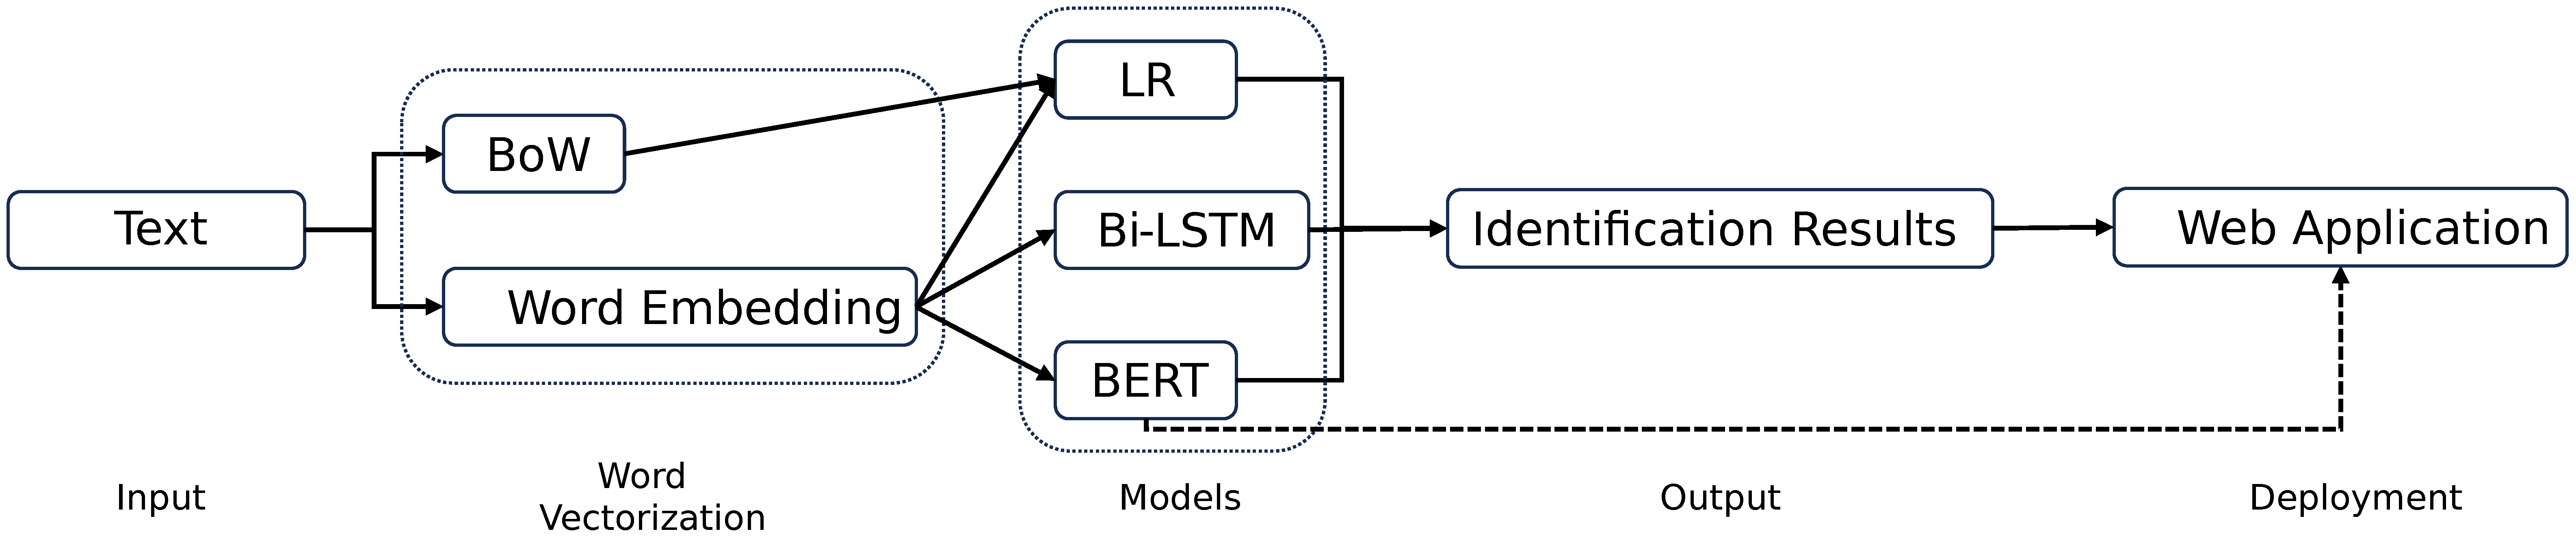
\includegraphics[width=0.9\linewidth]{../img/flow.eps}
      \caption{Workflow of the Project}
      \label{fig:flow}
\end{figure}

% -----------------------------------------------------------------------------

\chapter{Related Work}
\label{chap:background}
\noindent
Natural language processing (NLP) technology is currently developing at a rapid pace, and social network is becoming an indispensable part of people's daily lives as a means of expressing their inner thoughts. Research indicates that introverts are highly inclined to engage in online communication, which encourages more self-expression. An increasing number of capturable texts containing suicidal ideation are appearing on social media, prompting significant interest among scholars in computer science and psychology in conducting mental health research through internet or social network-based platforms.

\section{Identification of Suicidal Ideation}
\noindent
Suicide prevention and control are most effective when the at-risk individuals can be identified timely, which relies on an accurate evaluation of the suicidal tendencies. It has been found that many individuals contemplating suicide would usually reveal their intentions through speech, writing or specific behaviours before committing suicide\cite{smith2008revisiting}.

In early stages of suicide risk assessment, researchers utilized a single psychological scale to measure the risk of suicide, which is a method to quantify internal states into structured textual information\cite{Ghorashi2012AFP}. Although some results have been achieved\cite{sebastiani2006sentiwordnet}, a single scale may not comprehensively reflect the psychological state of an individual, especially suicide is still a very complex behaviour. Further more, the purposefulness of the questions in the scale can be easily detected by the subjects, leading to resistance or concealment of their true feelings\cite{world2014preventing}. Therefore, if the suicidal person choose to hide their intentions, it is easy to cause inaccurate outcomes.

Nowadays, due to the growing popularity of social media, some people utilize it as an anonymous "tree hole" to share their struggles and feelings. Therefore text analysis\cite{fursich2009defense} from online platforms is becoming a mainstream method.

Text analysis of social media content offers a potentially more comprehensive approach to suicide risk assessment. It enables examination of a broader range of expressions that may not be captured through traditional psychological scales. By applying NLP techniques and sentiment classification, it is possible to identify patterns and indicators of suicide ideation within textual data. This method can be particularly useful in detecting subtle features that may not be apparent through direct questioning or a single assessment scale.

\section{Word Vectorization}
\noindent
In NLP tasks, models rely on word vectorization techniques to transform textual data into input features. Word vectorization is a technique for modelling language and performing feature learning. Specifically, an individual word in a vocabulary is converted into a vector of real numbers, being utilized as input features to an model. Word vectorization methods can be classified into three categories: discrete representation, distributed representation, and dynamic pre-trained model representation.

\subsection{Discrete Representation}
\noindent
One-Hot encoding\cite{chren1998one} is a technique commonly used for discrete text representation, which a V-dimensional vector is utilized to represent each word, with $V$ being the total number of unique words contained in all documents. For each word, its corresponding dimension in the vector is set to $1$ and the remaining dimensions are set to $0$, thus providing a unique discrete vector representation for each word. However, the cosine similarity of each word vector is $0$. The method does not take into account the semantic relationships between words. 

The bag-of-words (BoW) model is proposed on the basis of One-Hot encoding, where a collection of text is represented by a two-dimensional vector of size $N \ast V$, where $N$ represents the number of samples and $V$ represents the size of the vocabulary list. Each row of the matrix corresponds to a vector representation of one sample, with each element indicating how many times a word appears in the current sample. 

As the research continues, the shortcomings of the BoW model are gradually revealed. Since the BoW model only distinguishes individual words and records the number of times each word occurs, disregarding the word order, it is unable to capture the relationships between words\cite{suresh2017multilevel}. In addition, the dimension of the word vectors is determined by the size of the vocabulary, leading to dimension disaster\cite{bengio2013representation} and sparse vectors, especially with large datasets.

\subsection{Distributed Representation}
\noindent
The distributed representations introduced by Hinton et al.\cite{hinton1986learning} are founded on the distributional assumption, which posits that a word's meaning is shaped by the words surrounding it. This assumption suggests that words with the similar context tend to have similar meanings, thereby leading to group them together. Bengio et al. obtained Neural Network Language Models (NNLM) to generate word vectors by learning both the distributed representation of each word and the likelihood function of the word sequences.\cite{bengio2000neural} This pioneering work paved the way for researchers to capture semantic and syntactic information. In 2007 Hinton et al. obtained Log-Bilinear (LBL) word vectors by improving Bengio's language model.\cite{mnih2007three} The following year, Collobert et al. introduced the C\&W model\cite{collobert2008unified}, which is a pre-trained word embedding model based on a deep learning model. This groundbreaking work has inspired many research in the field.

In 2013, Mikolov et al. proposed Word2Vec\cite{mikolov2013efficient}, building upon the foundations laid by the NNLM and C\&W models, which includes two main architectures: Continuous Bag-of-Words (CBOW) and Skip-gram models. These architectures aim to obtain word vectors quickly and efficiently by borrowing and simplifying the original models. In 2014, Pennington et al. proposed Global Vectors for Word Representation (GloVe) model\cite{pennington2014glove}, which presents a novel approach to word vector representation. GloVe combines both the traditional global matrix representation method and the local contextual word vector representation method trained by neural networks. Unlike previous methods that primarily focus on local context, GloVe leverages global word co-occurrence statistics to train the word vector model, providing a comprehensive representation of word semantics.

The above word vectorization models are obtained by training neural networks to capture either local context or global word vector representations, so they can excel in representing the semantic relationship between words than the traditional two-dimensional representation based on statistics. 

However, there are still some limitations of distributed representation. Both methods mentioned above use static way to represent text features, resulting in word embedding representation remain constant regardless of the context. But the same word may have different meanings in different contexts. Consider the word "apple", which sometimes represents a fruit, but sometimes represents electronic products, leading to ambiguity in meaning. This approach cannot effectively solve the issue of multiple meanings of words.

\subsection{Dynamic Pre-trained Model Representation}
\noindent
To address the challenge of inaccurate text representation, dynamic pre-trained model representation has been proposed as a promising solution. This approach involves pre-training on a large scale of text data, followed by fine-tuning on the specific downstream task to achieve diverse representations of the same word in different contexts. 

Peters et al.\cite{peters2018deep} proposed Embeddings from Language Models (ELMO). While Radford et al.\cite{radford2018improving} proposed the Generative Pre-Training (GPT) model GPT utilizes the decoder structure of Transformers\cite{vaswani2017attention}, but it is deficient in the text encoder method. In response to the limitations of the GPT model, Devlin et al.\cite{devlin2018bert} proposed Bidirectional Encoder Representations from Transformers (BERT). BERT addresses the shortcomings of GPT by utilizing a bidirectional approach, which allows it to capture contextual information more effectively. This bidirectional functionality permits BERT to consider not only the words that come before but also those that follow, thereby generating word representations that are more contextually informed. As a result, BERT achieves an enhanced context understanding and improved performance across various NLP tasks.

\section{Conventional Machine Learning}
\noindent
Machine learning can be categorized into two main subtypes: conventional machine learning and deep learning. Conventional machine learning starts from observation samples and tries to discover the complex laws behind them to achieve the prediction of future data trends. Statistics is a fundamental theoretical topic of conventional machine learning algorithms, which has gained wide application in several computer fields, including natural language processing, speech recognition and image processing. Related algorithms include Logistic Regression (LR), Hidden Markov Methods (HMM), Support Vector Machines (SVM), K Nearest Neighbours (KNN), Bayesian Methods, Decision Trees etc., mainly utilized for classification and regression tasks in the case of limited samples.

The main process of sentiment classification based on traditional machine learning is as follows. Firstly, the collected text data are labelled and processed to form a training set. Subsequently, the processed data undergo feature extraction. Following this, an appropriate supervised learning model is selected for training. Finally the trained model is able to predict the sentiment of unseen, new samples.

Pang et al. in 2002 first proposed the use of standard machine learning methods in solving emotion classification problems, with Naive Bayes, Maximum Entropy and SVM. And the experimental results show that SVM has the best effect among these methods. But these methods do not perform as well as in customary subject related classification.\cite{pang2002thumbs} B. Aliman et al. used several different models for binary sentiment analysis of tweets. The results show that Logistic Regression model outperforms SVM and Naive Bayes for the prediction of potential mental health crisis. \cite{aliman2022sentiment}

Despite the fact that conventional machine learning methods have achieved successes on some datasets and their ability to reduce labor costs. However, there are still some limitations in feature extraction, which makes it difficult to effectively extract features and mine deep semantics.

\section{Deep Learning}
\noindent
In recent years, with advancements in computer hardware performance, deep learning was first introduced by Hinton et al.\cite{hinton2006reducing} as a solution to the shortcomings of conventional machine learning methods. The core of deep learning is its backpropagation algorithm. Unlike conventional machine learning methods, deep learning methods can efficiently extract deeper semantics from text, resulting in significant improvements in performance. Thus deep learning approaches have dominated the field of NLP.

Currently the mainstream deep learning networks are: Convolutional Neural Networks (CNN)\cite{chua1998cnn} and Recurrent Neural Networks (RNN)\cite{socher2011parsing}. CNN excels in extracting static features from text and capturing regional information. KIM firstly introduced CNN into text processing tasks. With pre-trained word vectors from Google News, significant advancements were achieved in sentence-level text sentiment classification.\cite{2014Convolutional} 

However, CNN mainly focuses on sequence features in the text space, and cannot effectively capture dependencies within time-series data. Therefore, RNN, which is mainly designed for processing time-series data, is introduced to capture the dependencies between words, thereby facilitating the extraction of global information of text. RNN consists of multiple neurons that compute sequentially, where each neuron's input contains the output of the previous neuron, which gives the network a memory capability and the ability to handle variable length sequences.

\subsection{LSTM}
\noindent
However, when dealing with excessively long sequences, the RNN may suffer from gradient vanishing or gradient explosion, thus failing to solve the problem of long-range dependency. Hochreiter et al. improved on the RNN and proposed Long Short-Term Memory (LSTM).\cite{hochreiter1997long} Forget gates are used to regulate the retention and discarding of information\cite{greff2016lstm}, mitigating the limitations of traditional RNN and enhancing the capacity to capture long-range dependency. Tang et al. applied the LSTM to aspect-level sentiment analysis.\cite{tang2015target}

Traditional LSTM can only utilize the information of previous moments to predict current moments' information, but information from current moment may also be related to a future moment. To address this problem, bidirectional LSTM (BiLSTM) model was proposed, combining the outputs of the lstm units in both forward and backward directions and also leveraging contextual information. Experiments have demonstrated that BiLSTM models are usually more effective in dealing with contextual information compared to LSTM models that are unidirectional.\cite{hameed2019computationally}

\subsection{BERT}
\noindent
Bidirectional Encoder Representations from Transformers(BERT) was first proposed by Devlin et al. on the Google AI Language team.\cite{devlin2018bert}, represents a groundbreaking language representation model. Unlike traditional unidirectional language models, BERT aims to pre-train deep bidirectional representations by considering both left and right contexts. This model ushers a new era of large-scale pre-training based language models that significantly advances the field of NLP.

BERT mainly consists of multiple Transformers encoders, and each layer contains self-attention mechanism and feed-forward neural network.\cite{vaswani2017attention} By pre-training on extensive datasets and fine-tuning the BERT model, deep bi-directional linguistic representations are generated, which can be used in different NLP downstream tasks. Research by Bilal et al. employed BERT for sentiment classification\cite{bilal2023effectiveness}, Qu et al. utilized BERT for question-answering tasks\cite{qu2019bert}, and Miller et al. applied BERT for summarising texts\cite{miller2019leveraging}. The powerful advantages of pre-trained models have led increasing scholarly interest in NLP research with BERT.

Furthermore, scholars have introduced many variant models based on BERT to target improvements in diverse tasks and scenarios. RoBERTa, proposed by Facebook AI in 2019\cite{liu2019roberta}, improves the performance of the model with a larger vocabulary list, extended training sequences, augmented data, and diverse pre-training tasks. DistillBERT, introduced by Hugging Face in 2019\cite{sanh2020distilbert}, is a simplified version of BERT that approximates the performance of BERT with a smaller, faster model by distilling key information from BERT through knowledge distillation techniques. Additionally, BART, proposed by Facebook AI in 2019\cite{lewis2019bart}, adopts the BERT architecture for sequence-to-sequence tasks such as text summarization and text generation.

\section{Explainable AI}
\noindent
As artificial intelligence continues to evolve, there is growing interest in understanding the reasoning and decision-making processes behind AI systems. Although the accuracy in predictions is important, there is also a desire for models to provide explanations for the outputs.\cite{doshi2017towards} But with the emergence of new algorithms and increasingly complex model structures, the interpretability of the model gradually decreases. XAI was first proposed by Van et al.\cite{van2004explainable} to explain the behaviour of AI in simulation games. DARPA proposed the eXplainable AI (XAI) project\cite{gunning2019darpa}, with the goal of maintaining high performance while also being understandable and trustworthy to humans. Yeung et al.\cite{2021Enhancing} regarded XAI as "an innovation that opens the black box" and "a picking station for creating models and techniques". XAI allows humans to gain insight into how decisions are made and enabling them to trust and interact with these systems more effectively.

Different scholars have various opinions about explainability. Gunning et al.\cite{gunning2019xai} believe that explainability is to make behaviour more comprehensible to humans by providing explanations. Das et al.\cite{das2020taxonomy} define it as a metric for assessing the degree to which humans understand the reasons behind the decisions made by a model. Duval et al.\cite{duval2019explainable} assert that XAI should explain not only what the model has done, but also its current actions and future intentions. Despite these differing viewpoints, the goal of XAI is to empower humans to better understand and improve their models.

Current research on model explainability can be broadly categorized into two main approaches: model-based and model-independent methods.

Model-based methods are tailored to specific models and rely on the internal structure of the model for explanation. DeepLIFT\cite{shrikumar2017learning} decomposes the predictions of a neural network for a specific input by back-propagating the contributions of all the neurons in the neural network to each input variable, and is mainly used for the prediction of Deep Neural Network (DNN). The Layer-wise Relevance Propagation (LRP) algorithm\cite{bach2015pixel} assigns importance to neurons in each layer based on their correlation with the output of the network. The neurons with higher correlation have more influence and importance on the output of the network.

On the other hand, model-independent methods are applicable to a wide range of models and provide consistent interpretations irrespective of the model architecture. Partial Dependency Graphs, proposed by Friedman\cite{friedman2001greedy}, describes how features affect the model predictions, and can identify whether there is a linear correlation between the features and the labels. The Individual Conditional Expectation method\cite{goldstein2015peeking} portrays the relationship between each individual prediction and a single variable, offering a local explanation. Local Interpretable Model-agnostic Explanations (Lime), introduced by Ribeiro et al.\cite{ribeiro2016should}, explains individual instance predictions of black-box models. SHapley Additive exPlanations (SHAP) is a widely used model-independent method proposed by Lundberg and Lee\cite{lundberg2017unified}, which calculates the contribution of each feature to a prediction based on optimal Shapley values in game theory\cite{1953A}. KernelSHAP\cite{lundberg2017unified} and TreeSHAP\cite{lundberg2020local} are common variants of SHAP, and they are often used for explaining models and feature selection\cite{marcilio2020explanations}.

\section{Performance Metrics}
\noindent
Model evaluation metrics are very important for model selection to predict the model's capacity to classify unseen data, and models that classify well are of practical importance. 

Confusion matrix\cite{1997Selecting} is a tabular representation to show the performance of a classification model, and can count the number of samples that are correctly or mistakenly classified into each category. The confusion matrix is defined in Figure \ref{fig:confusion matrix}.

\begin{figure}[h]
      \centering
      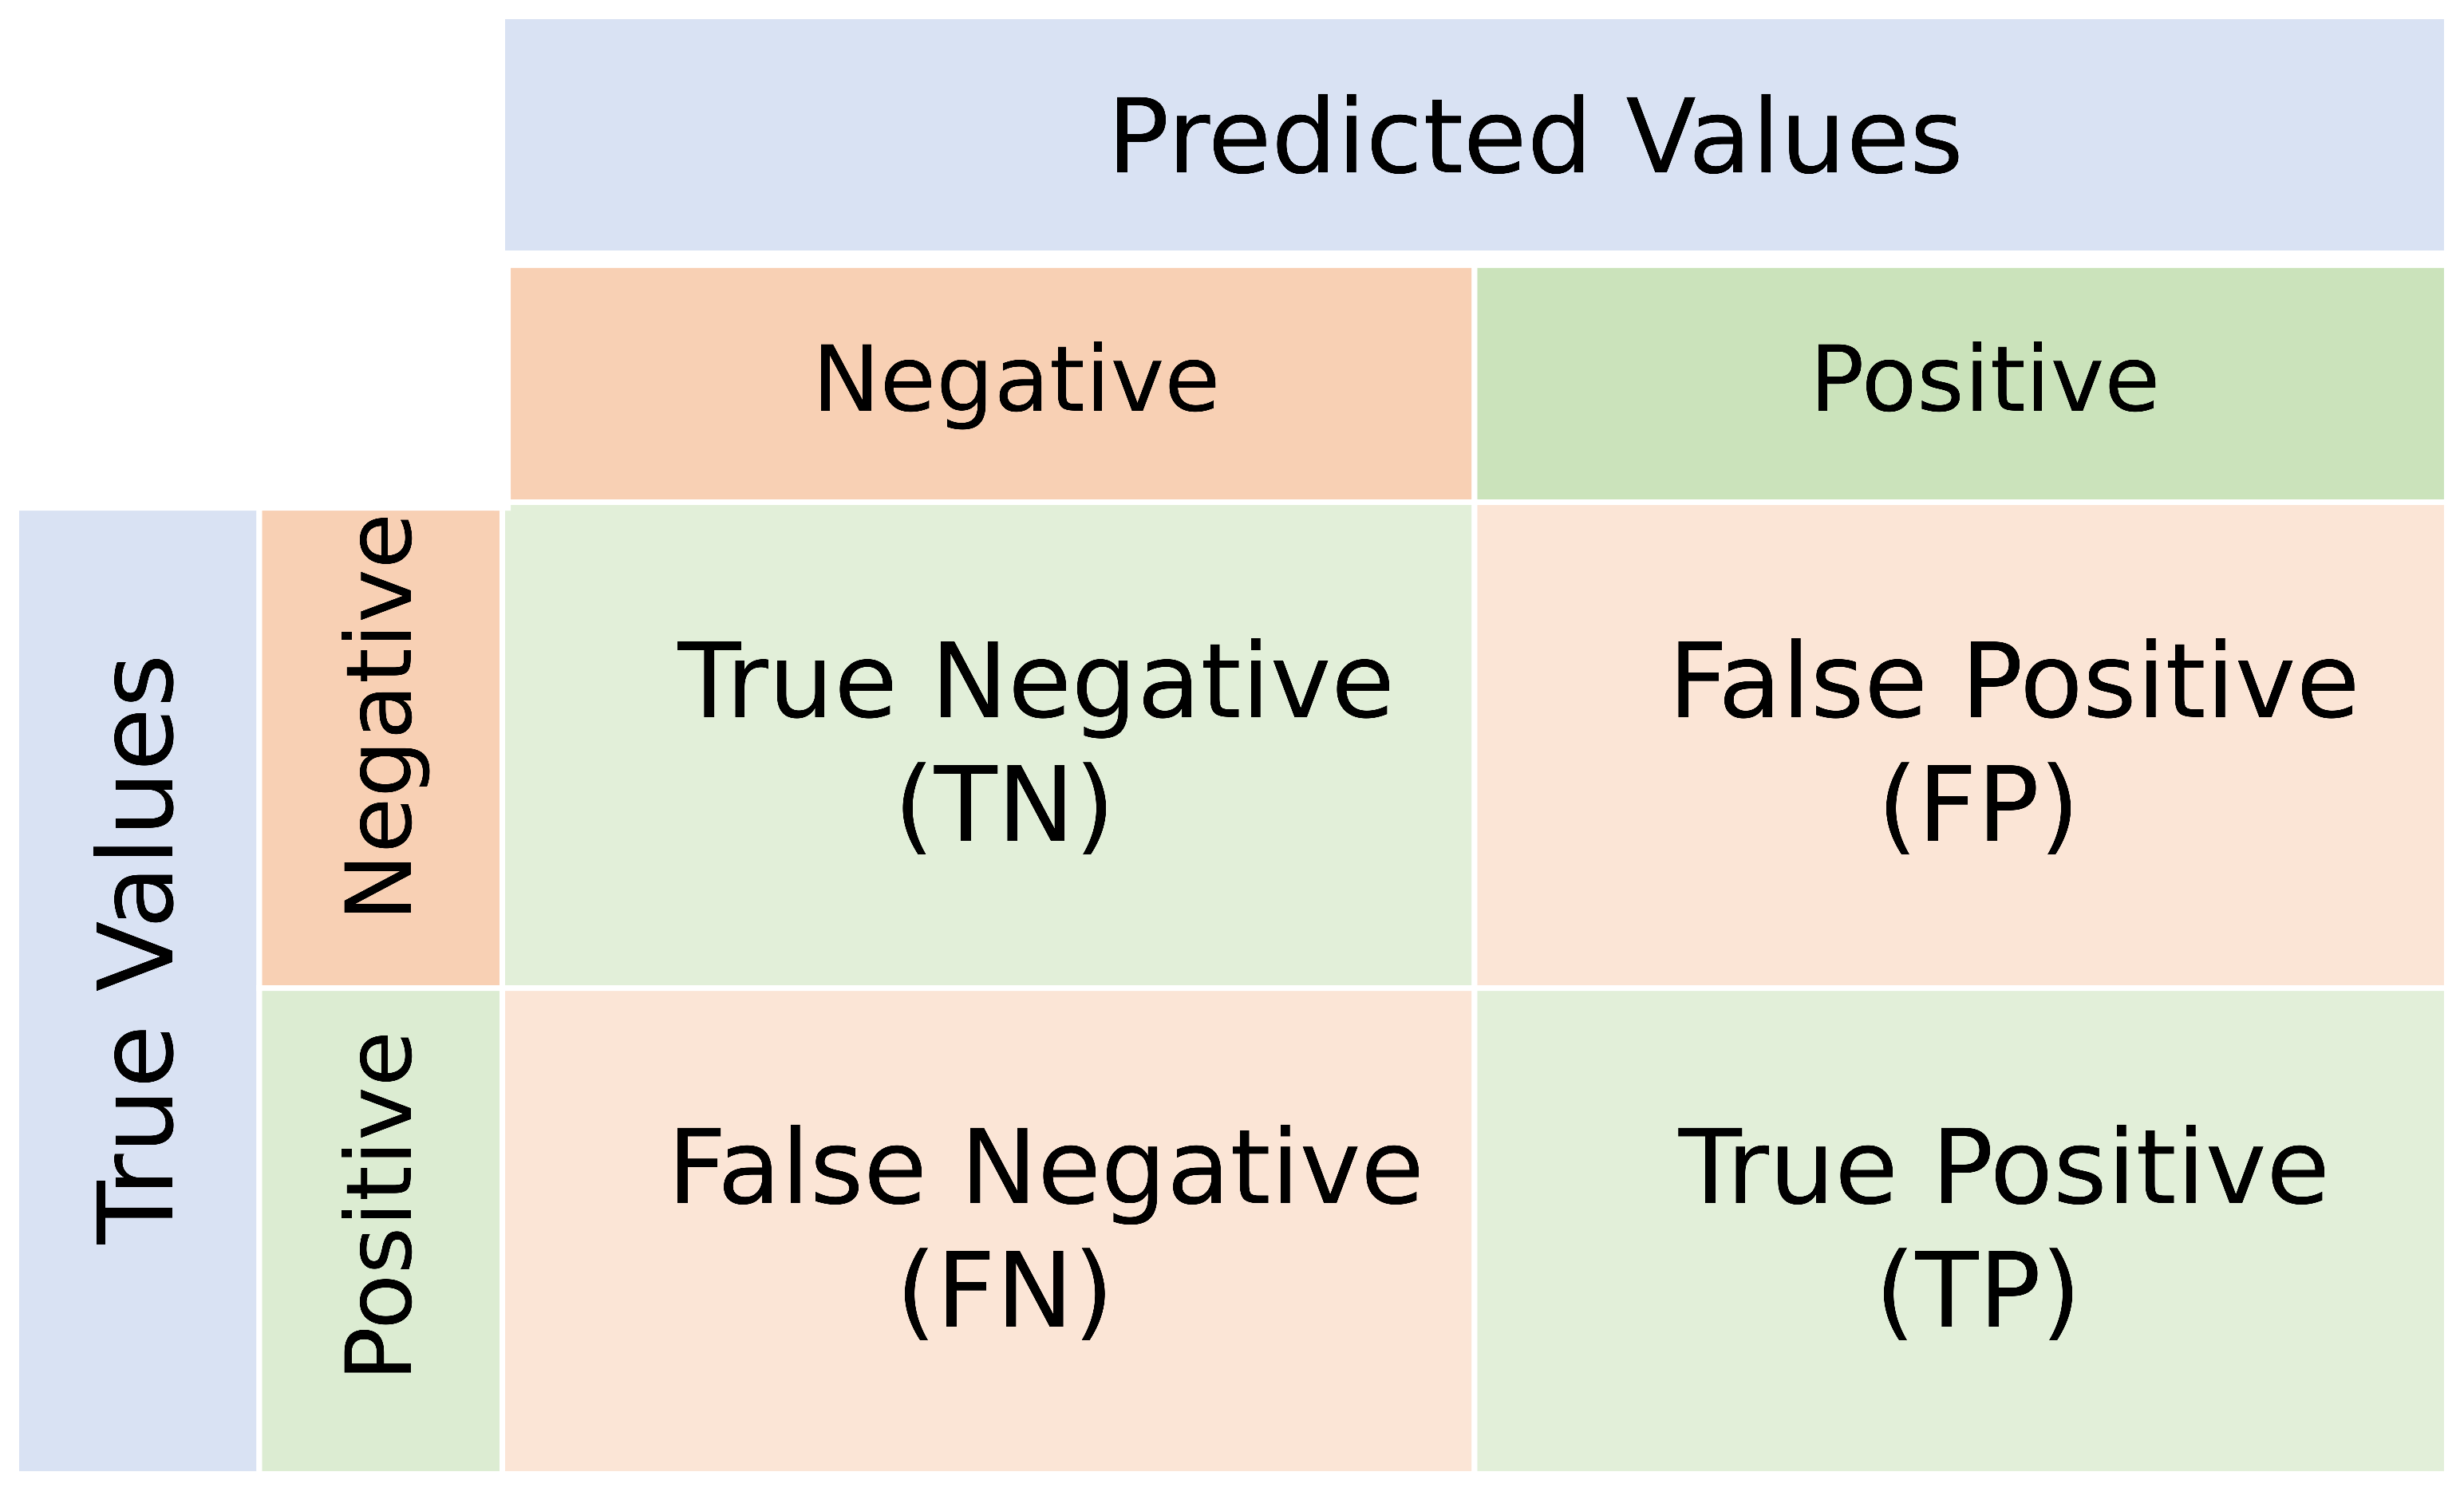
\includegraphics[width=0.6\linewidth]{../img/confusion matrix.eps}
      \caption{Confusion Matrix}
      \label{fig:confusion matrix}
\end{figure}

The confusion matrix is constructed based on the predicted results made by the classifier and the true labels of the samples. It provides a breakdown of the samples into four categories:

\begin{itemize}
      \item True Positive (TP): the quantity of positive examples classified accurately
      \item False Positive (FP): the quantity of actual negative examples classified as positive
      \item True Negative (TN): the quantity of negative examples classified accurately
      \item False Negative (FN): the quantity of actual positive examples classified as negative
\end{itemize}

Accuracy, precision, recall and F1 score are used as performance metrics to evaluate the model. 

Accuracy is the proportion of samples correctly predicted by the model to the total samples. It is obtained by quoting the number of correct samples in the prediction with the number of overall samples.

\begin{eqnarray}
      Accuracy = \frac{TP + TN}{TP + TN + FP + FN}
      \label{acc}
\end{eqnarray}

Precision measures the proportion of correctly predicted positive samples to the total number of positive predictions made by the model. It assesses the model's ability to avoid false positive predictions.

\begin{eqnarray}
      Precision = \frac{TP}{TP + FP}
      \label{pre}
\end{eqnarray}

Recall is the proportion of the number of positive samples correctly predicted by the model to the number of all positive samples in the dataset. It evaluates the model's ability to identify all positive samples.

\begin{eqnarray}
      Recall = \frac{TP}{TP + FN}
      \label{rec}
\end{eqnarray}

The F1 score is the harmonic mean of the precision and recall. It provides a balanced measure of a model's performance by considering both precision and recall simultaneously.

\begin{eqnarray}
      \begin{aligned}
            Precision &= \frac{2\ast Precision \ast Recall}{Precision + Recall} \\
                      &= \frac{2\ast TP}{2 TP + FP + FN}
      \end{aligned}
      \label{f1s}
\end{eqnarray}


% -----------------------------------------------------------------------------

\chapter{Baseline Model}
\label{chap:execution1}
\noindent
This chapter will cover an approach to sentiment classification based on baseline model. The initial section outlines how to pre-process the data, and transform textual data into a format compatible with the model. Subsequently, the second section contains an explanation of the baseline model. Moving forward, the third section tries to enhance the model performance by optimising the data processing part based through the utilization of word embedding. Following this, the fourth section evaluates the model through the analysis of the performance metrics. Finally, the last section includes the explanation of the model, dissecting the factors contributing to both its good and bad performances.

\section{Preprocess Data}
\noindent
Since algorithms can only handle numeric data, data preprocessing is essential to enable text data to be received by the model and facilitate learning features. Raw text often contains a lot of redundant and repetitive information, while data preprocessing can help the algorithm to focus on the core content of the text, which improves the accuracy of the algorithm.

\subsection{Exploratory Data Analysis}
\noindent
Firstly, the entire dataset undergoes the test to see whether it is balanced or not, and if there are any missing values. Alongside the length distribution within each category is analyzed. Upon dataset examination, it's revealed that the label consists of two categories: "suicide" and "non-suicide". The sample size of both categories is 116,037 entries, which is a balanced dataset with no missing values. However, there's significant variance in the average data length between categories. Figure \ref{fig:describe} depicts the relationship between sample length, in terms of the number of tokens, and sample numbers. 

\begin{figure}[h]
      \centering
      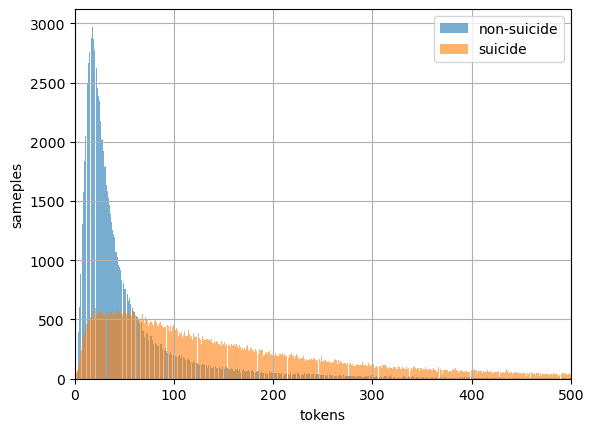
\includegraphics[width=0.6\linewidth]{../img/data_describe.png}
      \caption{Distribution of Data across Samples of Varying Lengths}
      \label{fig:describe}
\end{figure}

Notably, the average sample length in the "suicide" category exceeds that of the "non-suicide" category. The specific data is shown in the Table \ref{tab:describe}.

\begin{table}[h]
      \centering
      \begin{tabular}{ccccc}
            \hline
            class & count & mean length & min & max \\
            \hline
            suicide     & 116037 & 61.188  & 2 & 8220 \\
            non-suicide & 116037 & 202.662 & 1 & 9684 \\
            \hline
      \end{tabular}
      \caption{Data Description}
      \label{tab:describe}
\end{table}

Following the initial analysis, word clouds were generated for each of the two categories of data. A word cloud offers a visual depiction of word frequency. The more frequently a word occurs within the text being analysed, the larger that word is in the generated image. This visualization technique is increasingly being used as a simple tool for determining the focus of written material.\cite{atenstaedt2012word} Figure \ref{fig:word cloud} shows the word cloud of both "non-suicide"(Figure \ref{fig:word cloud}\ref{sub@wc_n}) and "suicide"(Figure \ref{fig:word cloud}\ref{sub@wc_s}) categories.

\begin{figure}[h]
      \centering
      \subfloat["non-suicide" Class]{
            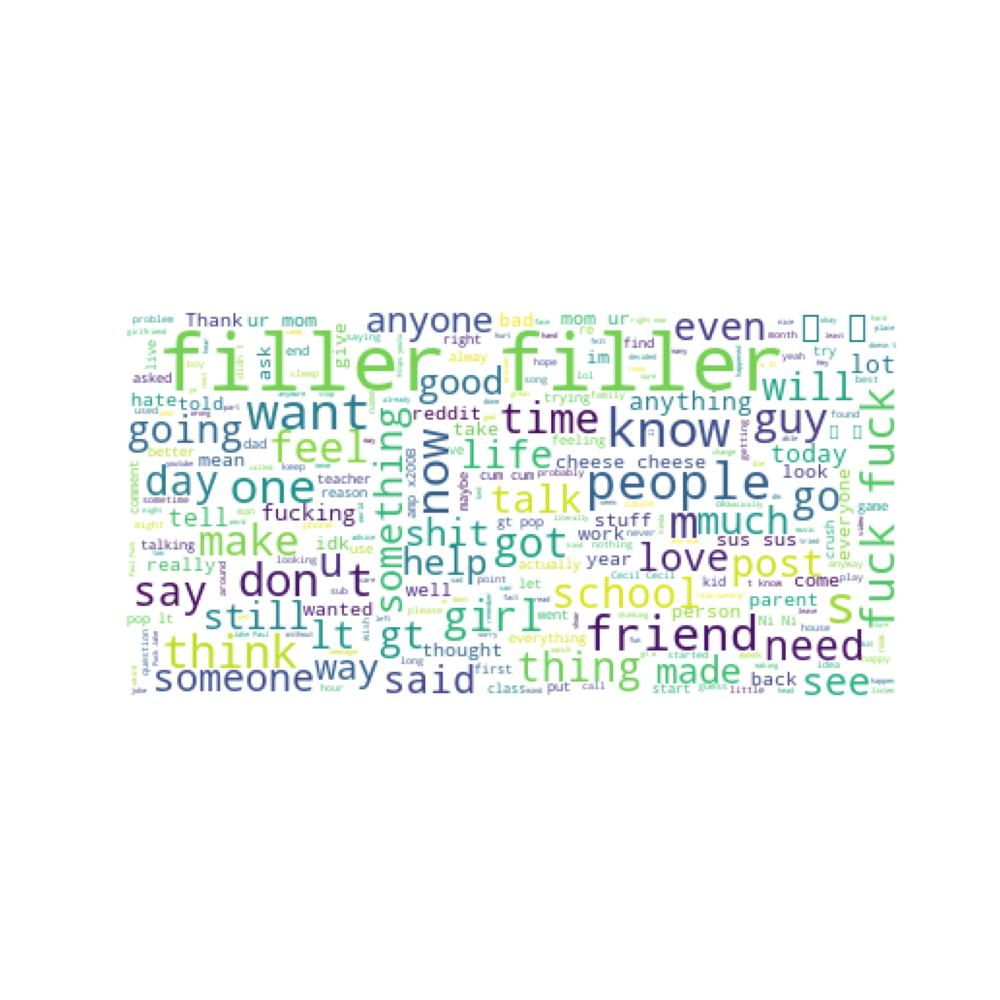
\includegraphics[width=0.44\linewidth]{../img/wc_nonsuicide.jpg}
            \label{wc_n}}
      \hfil
      \subfloat["suicide" Class]{
            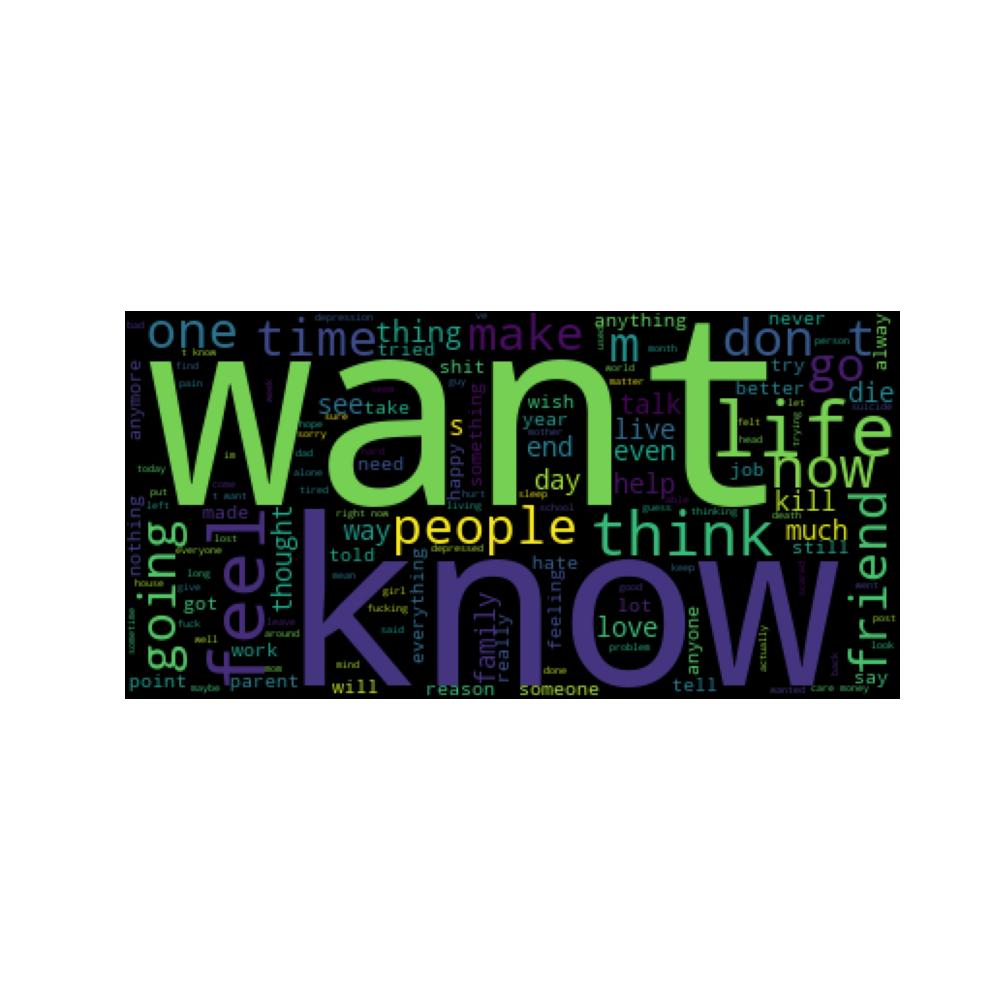
\includegraphics[width=0.44\linewidth]{../img/wc_suicide.jpg}
            \label{wc_s}}
      \caption{Word Cloud of both two Categories of Raw Texts}
      \label{fig:word cloud}
\end{figure}

\subsection{Data Cleaning}
\noindent
After performing exploratory data analysis, a general understanding of the data set has been obtained. The next step should be to preprocess the data.

Missing values can appear due to a number of factors, such as data entry errors, sensor failures, or human error. Common processing methods to deal with missing values include deleting, filling with special values, marking as a new class, and so on. The selection of a method depends on the characteristics of the dataset and the most appropriate method must be chosen accordingly. However, since there are no missing values in this dataset, this step is not required.

Given the presence of numerous abbreviations in the text, which may lead to interpretational confusion. Therefore it is essential to convert common abbreviations into their full forms. This can be handled with a dictionary structure in Python, containing common abbreviations and corresponding full forms. Each word in the text can then be iterated through regular expressions and the abbreviations contained in the dictionary are replaced.

What's more, the dataset may contain many unwanted content such as URLs, emojis, special symbols, etc. These are not conductive to semantic analysis of the text and may even interfere with the learning process of the model. Such content can be filtered out with regular expressions.

Finally, it is vital to remove the stopwords in the text. Stopwords are words that appear frequently in the text (e.g., "the", "is", "and") but contribute minimally to the meaning of the text. Removing these words can enhance text processing efficiency. Many organisations published their pre-made stopwords lists. Here the English stopword list provided by the NLTK library is used to remove stopwords from the dataset.

Subsequently, Figure \ref{fig:word cloud clean} shows the word cloud of the dataset extracted after data cleaning to compare the result before and after data cleaning.

\begin{figure}[h]
      \centering
      \subfloat["non-suicide" Class after Cleaning]{
            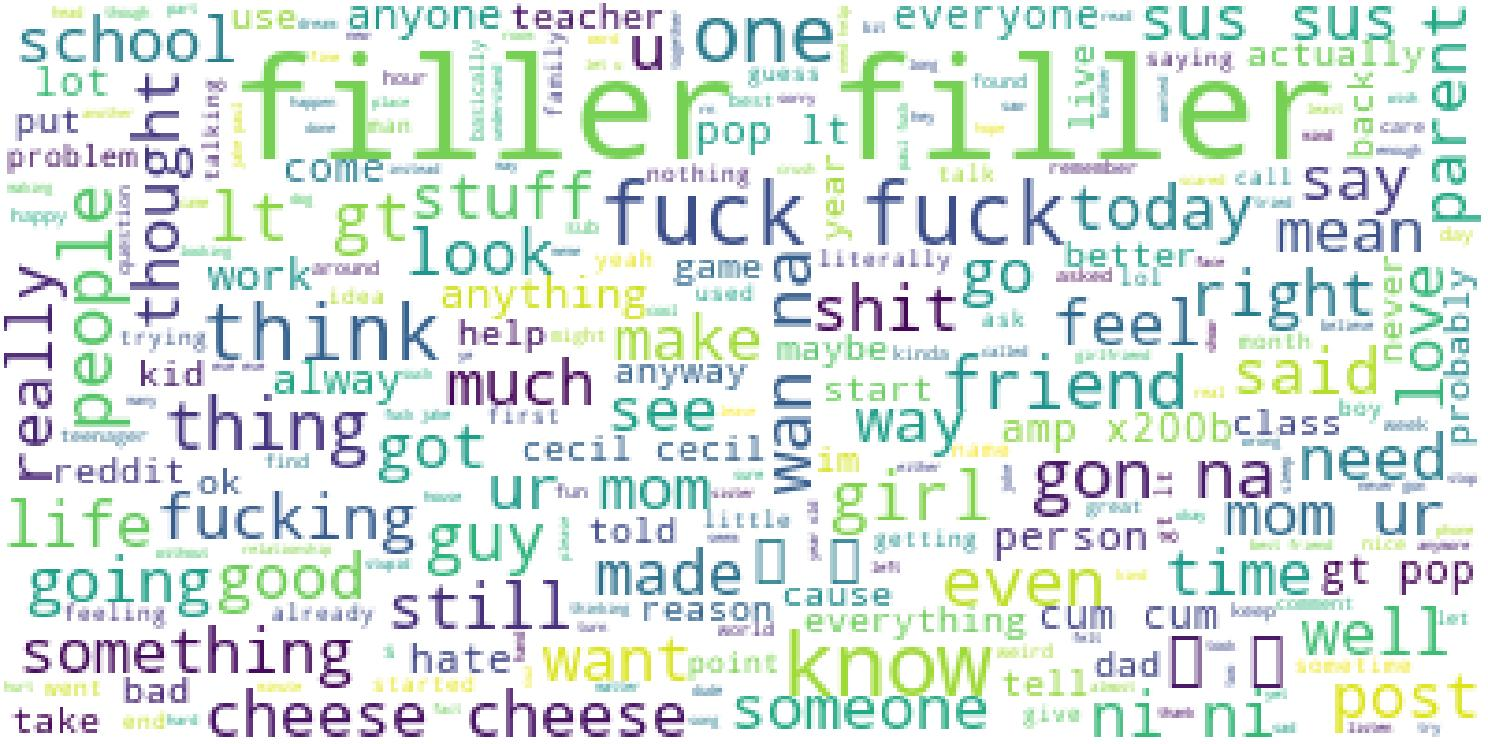
\includegraphics[width=0.44\linewidth]{../img/wc_nonsuicide_c.jpg}
            \label{wc_n_c}}
      \hfil
      \subfloat["suicide" Class after Cleaning]{
            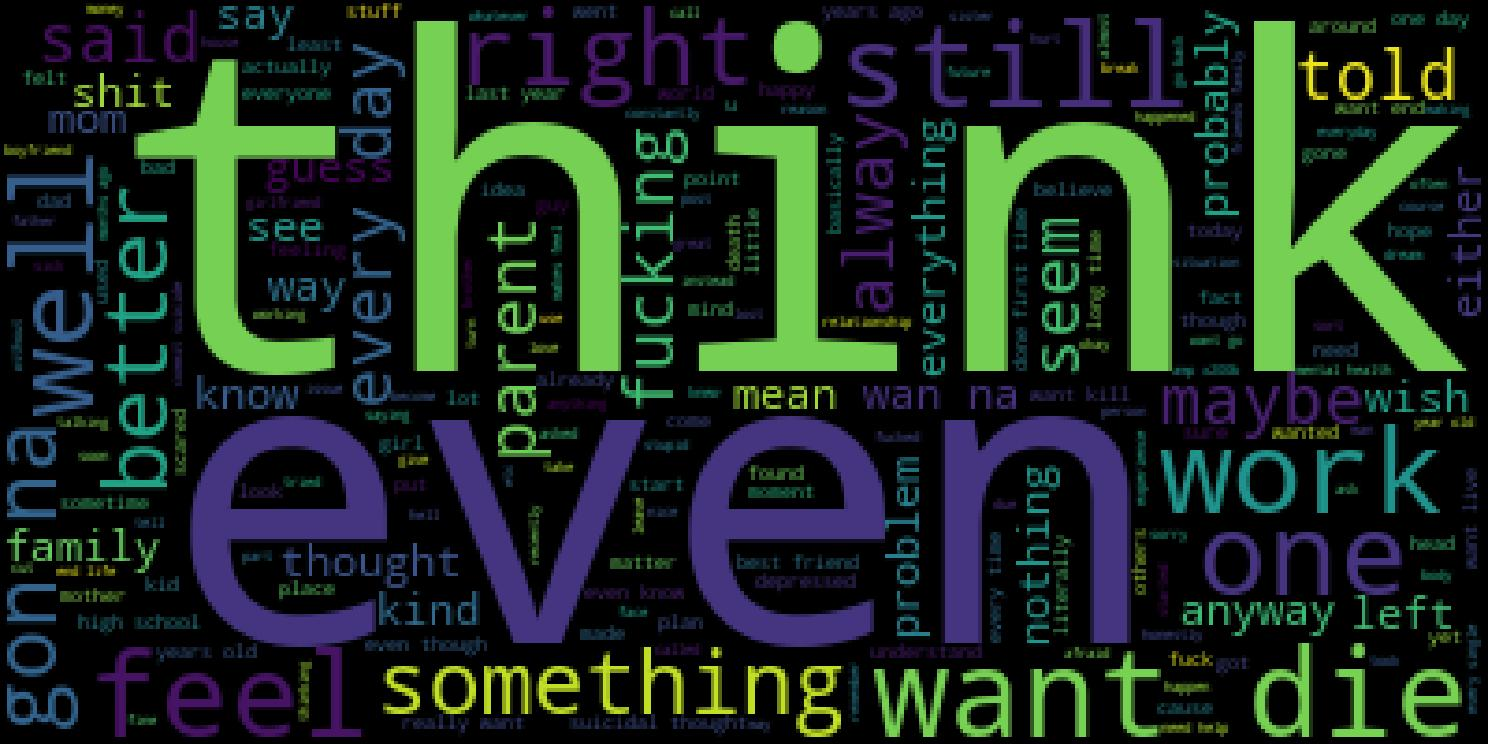
\includegraphics[width=0.44\linewidth]{../img/wc_suicide_c.jpg}
            \label{wc_s_c}}
      \caption{Word Cloud of both two Categories after Data Cleaning}
      \label{fig:word cloud clean}
\end{figure}

\subsection{Word Vectorization}
\noindent
After cleaning the dataset, the text needs to be vectorially represented. BoW model is one of the commonly used vector representation models among so many models. BoW model, based on one-hot encoding\cite{chren1998one}, is a simple yet powerful technique used in NLP for representing text data. It's based on the concept of treating text as a "bag" of individual words, disregarding grammar and word order, and focusing solely on word frequency. The workflow of the model is divided into the following steps:

\begin{enumerate}
      \item Tokenization: The first step is to break down the text into individual tokens. This process involves splitting the text into words based on whitespace characters.
      \item Vocabulary Creation: Next, a vocabulary is created by compiling a list of unique words present in the entire dataset. Each unique word in the vocabulary becomes a feature in the BoW model.
      \item Vectorization: For each document in the dataset, a vector is constructed where each element represents the frequency of a word from the vocabulary in that document. The length of the vector is equal to the size of the vocabulary, and the values are the counts of each words in a document.
      \item Sparse Representation: Since most documents only contain a small subset of the words in the vocabulary, the resulting vectors are typically sparse, meaning that most of the elements are zero.
\end{enumerate}

During implementation, the maximum number of features can be set to prevent excessive dimensionality and to speed up processing. Finally a sparse matrix representing the number of occurrences of all the words in dataset will be obtained as the word vector passed to the model.

\section{Logistic Regression}
\noindent
After the data pre-processing step, a vector-like representation of the data is obtained, which can be served as the training and testing data for the baseline model. Here, logistic regression is used as the baseline model. Logistic regression is a classification method in the field of statistics and machine learning. The goal of logistic regression is to predict the probability of an event occurring, achieved through a combination of linear regression and an activation function.

As a generalized linear regression algorithm, logistic regression initially employs a linear regression algorithm to model the relationship between the independent (features) and dependent (outcome) variables. The linear equation takes the following form:

\begin{eqnarray}
      z=b_0+b_1x_1+b_2x_2+\cdots+b_nx_n
      \label{Linear Regression}
\end{eqnarray}

Where $x_1,x_2,\cdots,x_n$ are the feature variables that influence suicide ideation, here representing different tokens mentioned earlier. $b_1,b_2,\cdots,b_n$ are the weight coefficient of each variable determining the extent how tokens impact on the results. The output $z$ is next passed to a logistic function that maps a linear result over the range of the real number domain to a value between $0$ and $1$, facilitating the classification task. The sigmoid function is most commonly used for this transformation, defined as:

\begin{eqnarray}
      p=\sigma(z)=\frac{1}{1 + e^{-z}}
      \label{Sigmoid Function}
\end{eqnarray}

Where $p$ represents the probability of being a "suicide" sample. The complete logistic regression formula can be obtained by combining the two formulas:
\begin{eqnarray}
      p=\frac{1}{1 + e^{-(b_0+b_1x_1+b_2x_2+\cdots+b_nx_n)}}
      \label{Logistic Regression}
\end{eqnarray}

After that, a threshold is determined to serve as a dividing line (usually 0.5), making the predicted probability converted into a binary outcome. If the predicted probability is greater than the threshold, the sample is classified to "suicide" class; otherwise, it is classified as a "non-suicide" sample.

Logistic regression iteratively updates the coefficients $b_1,b_2,\cdots,b_n$ through optimisation algorithms such as maximum likelihood estimation (MSE) or stochastic gradient descent (SGD). The objective is to adjust the coefficients so that the predictions of the model could be closer to the true values. This iterative optimization process continues until convergence, where the model parameters converge to their optimal values, leading to the best model performance.

\section{Improve with Word Embedding}
\noindent
Considering the large size of the dataset, the dimensionality of the BoW model escalates, resulting in what is commonly referred to as the "dimensional disaster". And it lacks the ability to capture relationships between words, which is poor for semantic extraction. While the word embedding approach offers a solution by mapping words to a fixed-dimensional vector space, which is much smaller than the vocabulary's dimension. This facilitates the evaluation of semantic proximity among various words in the vector space, while also encompassing contextual nuances to differentiate between disparate meanings of the same word across contexts. Consequently, word embedding is applied to try to improve the model performance.

As one of the current mainstream pre-training models, BERT is pre-trained with a large number of samples and has good performances in many tasks. Therefore the tokenizer and word embedding methods provided by BERT are used to process the text data.

\subsection{Tokenize}
\noindent
In order to help the model understand the text and discern each word within a sentence, a tokenizer is employed to break the text into small tokens, which are subsequently transformed into word vectors. 

While the previously mentioned BoW model typically separates tokens based on spaces, it encounters challenges with words exhibiting various forms, such as tense or plurality. Moreover, space is not used to segment words in many language like Chinese, so this method is not universally applicable. In order to improve the word tokenization method, the subword-based method is introduced. This method splits larger words into small subwords, mitigating the need to tokenize every word individually from an extensive dataset. For example, "transformer" can be segmented into "transform" + "er", which is more flexible and adaptive. 

BERT uses the WordPiece algorithm\cite{wu2016google}, one of the subword-based methods, for its tokenizer, segmenting the word "transformer" into "transform" + "\#\#er". The "\#\#" of the latter token indicates that it is part of the former word. To helping effectively utilizing BERT model in different NLP tasks, Bert Tokenizer adds some special tokens to the text:

\begin{itemize}
      \item\ [CLS]: Added at the beginning of a sequence, usually for classification tasks.
      \item\ [SEP]: Added at the end of a sequence to separate sentences or mark the end of a sentence pair.
      \item\ [PAD]: Used to fill the sequence to a uniform length.
      \item\ [UNK]: Used to represent words outside the BERT vocabulary, enhancing the model's generalisation of new words.
      \item\ [MASK]: Used in pre-training for masking language modelling tasks.
\end{itemize}

After the split, the tokeniser converts the text into a format that the BERT model can understand. This method returns a dictionary consisting of the following:

\begin{itemize}
      \item input\_ids: a sequence of ids for the token string, based on the vocabulary
      \item attention\_mask: indicates which tokens are valid and which are padded
      \item token\_type\_ids: sequences that distinguish different sentences in a sentence pair (if it is a sentence pair)
\end{itemize}

\subsection{Word Embedding}
\noindent
Like many other deep learning models in NLP, BERT processes the words in the text through the token embedding layer to convert them into word vectors. However, unlike conventional models, BERT has two additional embedding layers, the segment embedding layer and the position embedding layer. This unique architecture of the BERT embedding layer is depicted in the Figure \ref{fig:bert_embedding}.

\begin{figure}[h]
      \centering
      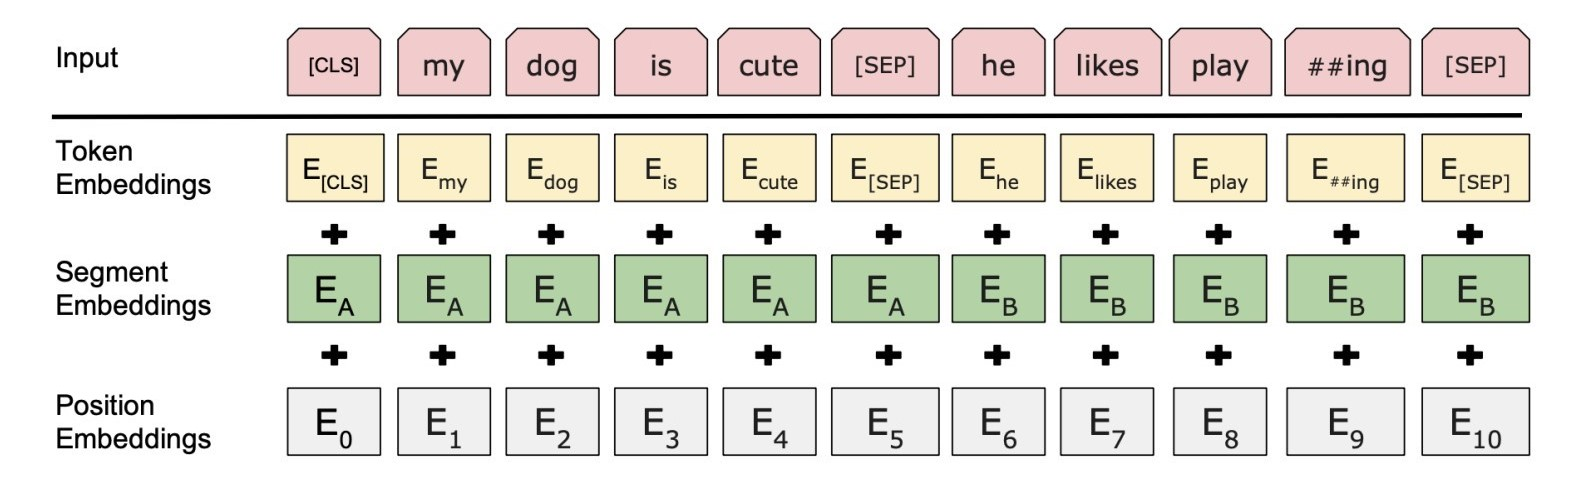
\includegraphics[width=0.6\linewidth]{../img/bert_embedding.jpg}
      \caption[BERT Input Representation]{BERT Input Representation.\cite{devlin2018bert}}
      \label{fig:bert_embedding}
\end{figure}

Token Embeddings: Encode the word IDs and convert them into fixed-dimensional vectors. In BERT, each word is typically transformed into a 768-dimensional vector representation by default. Suppose $batch\_size$ represents the size of a batch and $sen\_length$ represents the number of tokens in a sentence. After tokenization, the size of a batch of texts is $[batch\_size, sen\_length]$ and it becomes a three dimensional tensor with size $[batch\_size, sen\_length, 768]$ after embedding.

Segment Embeddings: Useful only when the input is a sentence pair, it helps BERT to distinguish whether a token belongs to the first sentence or the second sentence. Since only a single sentence is considered for determining suicide ideation, all elements in the output of this layer are $0$.

Position Embeddings: Facilitate BERT in learning the sequential order of input tokens. Because of Transformers' inability to handle sequence positions, position information need to be added manually to ensure proper sequence handling.

The three embedding results are summed without weights with a size of $[batch\_size, sen\_length, 768]$. BERT applies layer normalisation to adjust the resultant tensor\cite{pymars2020normalisation}, which contributes to the stability and efficiency of model training. Finally, BERT applies dropout technique to regularise the model and reduce the risk of overfitting.

\section{Baseline Model Performance}
\noindent
The dataset is split into a training set and a test set in the ratio of 8:2. The training set is utilized to train the model so that it can learn the relationships within the data, enabling the model to perform well on the target task. The test set is not involved in the training process and is reserved as unseen data. This separation simulates real-world scenarios where the model encounters new, unseen data for prediction. By evaluating the model's performance on the test set, its predictive capability under real-world conditions can be assessed.

To ensure the accuracy and reliability of the results, a stratified K-fold cross-validation approach is employed on the training set\cite{browne2000cross}. The entire training set is divided into $K$ equal-sized subsets, known as "folds". Moreover, each fold maintains the same proportion of samples in each category as in the original dataset, enhancing the robustness of performance estimates. During each iteration of the cross-validation process, one fold is selected as the validation set and the remaining serve as the training set to evaluate the model performance. This process is repeated $K$ times. Finally, the average performance metric of all $K$ iterations is calculated to get the generalisation ability of the model. In this experiment the value of $K$ is chosen as $5$. The structure of the cross validation process is showen in Figure \ref{fig:cross validation}.

\begin{figure}[h]
      \centering
      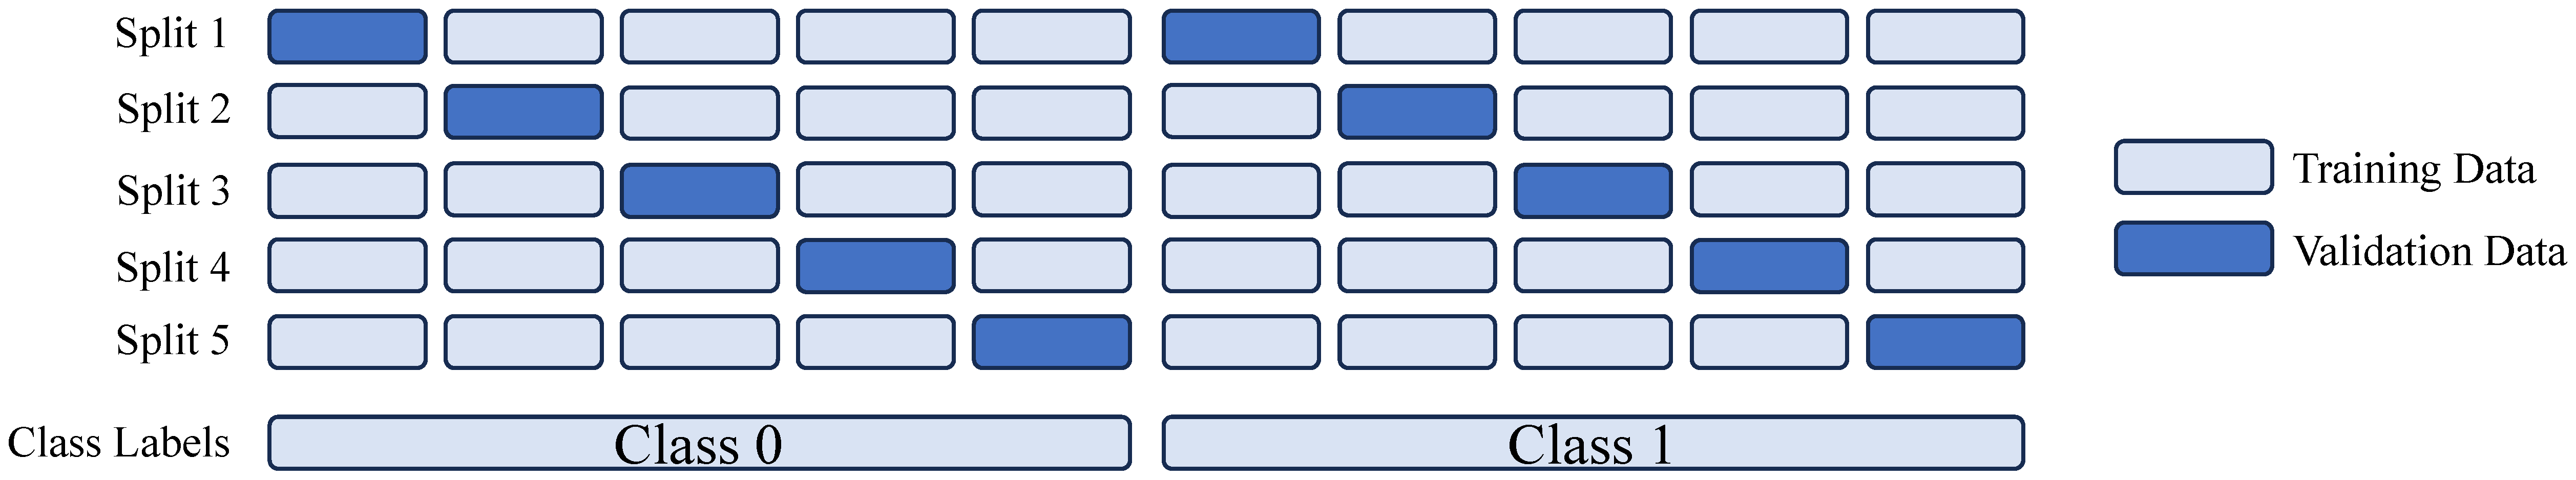
\includegraphics[width=0.7\linewidth]{../img/cv.eps}
      \caption{Stratified K-Fold Cross Validation}
      \label{fig:cross validation}
\end{figure}

After cross-validation, the average performance metrics of the two word vectorization methods on the logistic regression model are shown in the Table \ref{tab:baseline}. 

\begin{table}[h]
      \centering
      \begin{tabular}{cccccc}
            \hline
            Word Vectorization Method & Accuracy (\%) & Precision (\%) & Recall (\%) & F1 Score (\%) & Iteration \\
            \hline
            BoW model      & 93.26 & 95.13 & 91.18 & 93.11 & 691    \\
            Word Embedding & 73.34 & 75.00 & 70.02 & 72.42 & 1697   \\
            \hline
      \end{tabular}
      \caption{Performance Metrics of Different Word Vectorization Methods on Logistic Regression}
      \label{tab:baseline}
\end{table}

However, word embedding technique, which is supposed to contain more information, are not as effective as BoW models. The prediction performance on the test dataset is shown in Tabel \ref{tab:lrperformance}

\begin{table}[!h]
      \centering
      \begin{tabular}{c|cccc}
            \hline
            Model & Acc(\%) & Pre(\%) & Rec(\%) & F1(\%) \\
            \hline
            LR with BoW             & 93.51 & 95.56 & 91.28 & 93.37 \\
            LR with bert embedding  & 73.66 & 75.63 & 69.88 & 72.64 \\
            \hline
      \end{tabular}
      \caption{Performance Mertics of four Models}
      \label{tab:lrperformance}
\end{table}

\section{Baseline Model Explanation}
\noindent
For the BoW technique, since each token is treated as a separate dimension, the model prediction results can be interpreted by looking at the feature weights of the tokens. Table \ref{tab:weights} demonstrates a few tokens with substantial weights. The stranger word forms can likely be attributed to the manner in which the sample was collected. Specifically, the data collection process did not account for inter-sentence segmentation, treating the word at the end of a sentence as one word along with the "I" at the beginning of the next sentence. It can be seen that words with strong sentiment representations will have larger weights and have a greater impact on the model output.

\begin{table}[h]
      \centering
      \begin{tabular}{c|ccccc}
            Token  & helpi & diei  & anymorei & lifei & suicidei \\
            \hline
            Weight & 4.663 & 4.235 & 4.222    & 3.907 & 3.650
      \end{tabular}
      \caption{High Weight Tokens in LR with BoW}
      \label{tab:weights}
\end{table}

Word embedding technique maps words to a vector space of fixed dimensions, precluding a direct correspondence between feature values and individual words. Therefore, SHAP is applied to explain the model. The force plot above the text provides an overview of how tokens combine together to produce the model's output. The red features "pushing up" the model output and the blue features "pulling down" the output. Figure \ref{fig:lrshap} provide a degree of explanation of the model predictions.

\begin{figure}[!h]
      \centering
      \subfloat[False Positive Sample]{
            
\includegraphics[width=0.75\linewidth]{../img/LR_B_fp.png}
            \label{lr_fp}}

      \subfloat[False Negative Sample]{
            
\includegraphics[width=0.75\linewidth]{../img/LR_B_fn.png}
            \label{lr_fn}}
      \caption{Wrongly Predicted Samples Explained by SHAP}
      \label{fig:lrshap}
\end{figure}

The first sample can be found out to be discussing what is going on in the game. Despite the presence of numerous words that typically signal a non-suicidal context, in the end the model concludes with a suicide category. In the second sample, the model even categorizes many words with obvious negative emotions, such as "pain" and "freaking", as contributing to the non-suicide category. These observations highlight the shortcomings of LR in capturing the sophisticated semantic information encoded in word embedding, which can lead to completely opposed conclusions. This realization also motivates this project to replace the prediction model so as to effectively utilize the rich information in word embedding, thereby enhancing the accuracy and reliability of sentiment analysis.

% -----------------------------------------------------------------------------

\chapter{Deep Learning Model}
\label{chap:execution2}
\noindent
In this chapter, the process of improving the task with deep learning models will be covered. The initial section uses a model of RNN to optimise the task, offering insights into its foundational principles and the selection of hyperparameters. Subsequently, the second section leverages the current dominant large language model to further refine the optimization process.

\section{Recurrent Neural Network}
\noindent
Since logistic regression has a good performance on simpler features, but performs poorly with the complexity of word embedding methods. To address this limitation, word embedding requires further processing through more sophisticated algorithms. Considering the importance of understanding textual information, RNN is employed for learning features in texts. The memory unit of RNN (as shown in the Figure \ref{fig:rnn}) is able to retain information from previous time steps, which allows RNN to capture historical information, making it well-suited for sequential data processing tasks such as text classification. 

\begin{figure}[h]
      \centering
      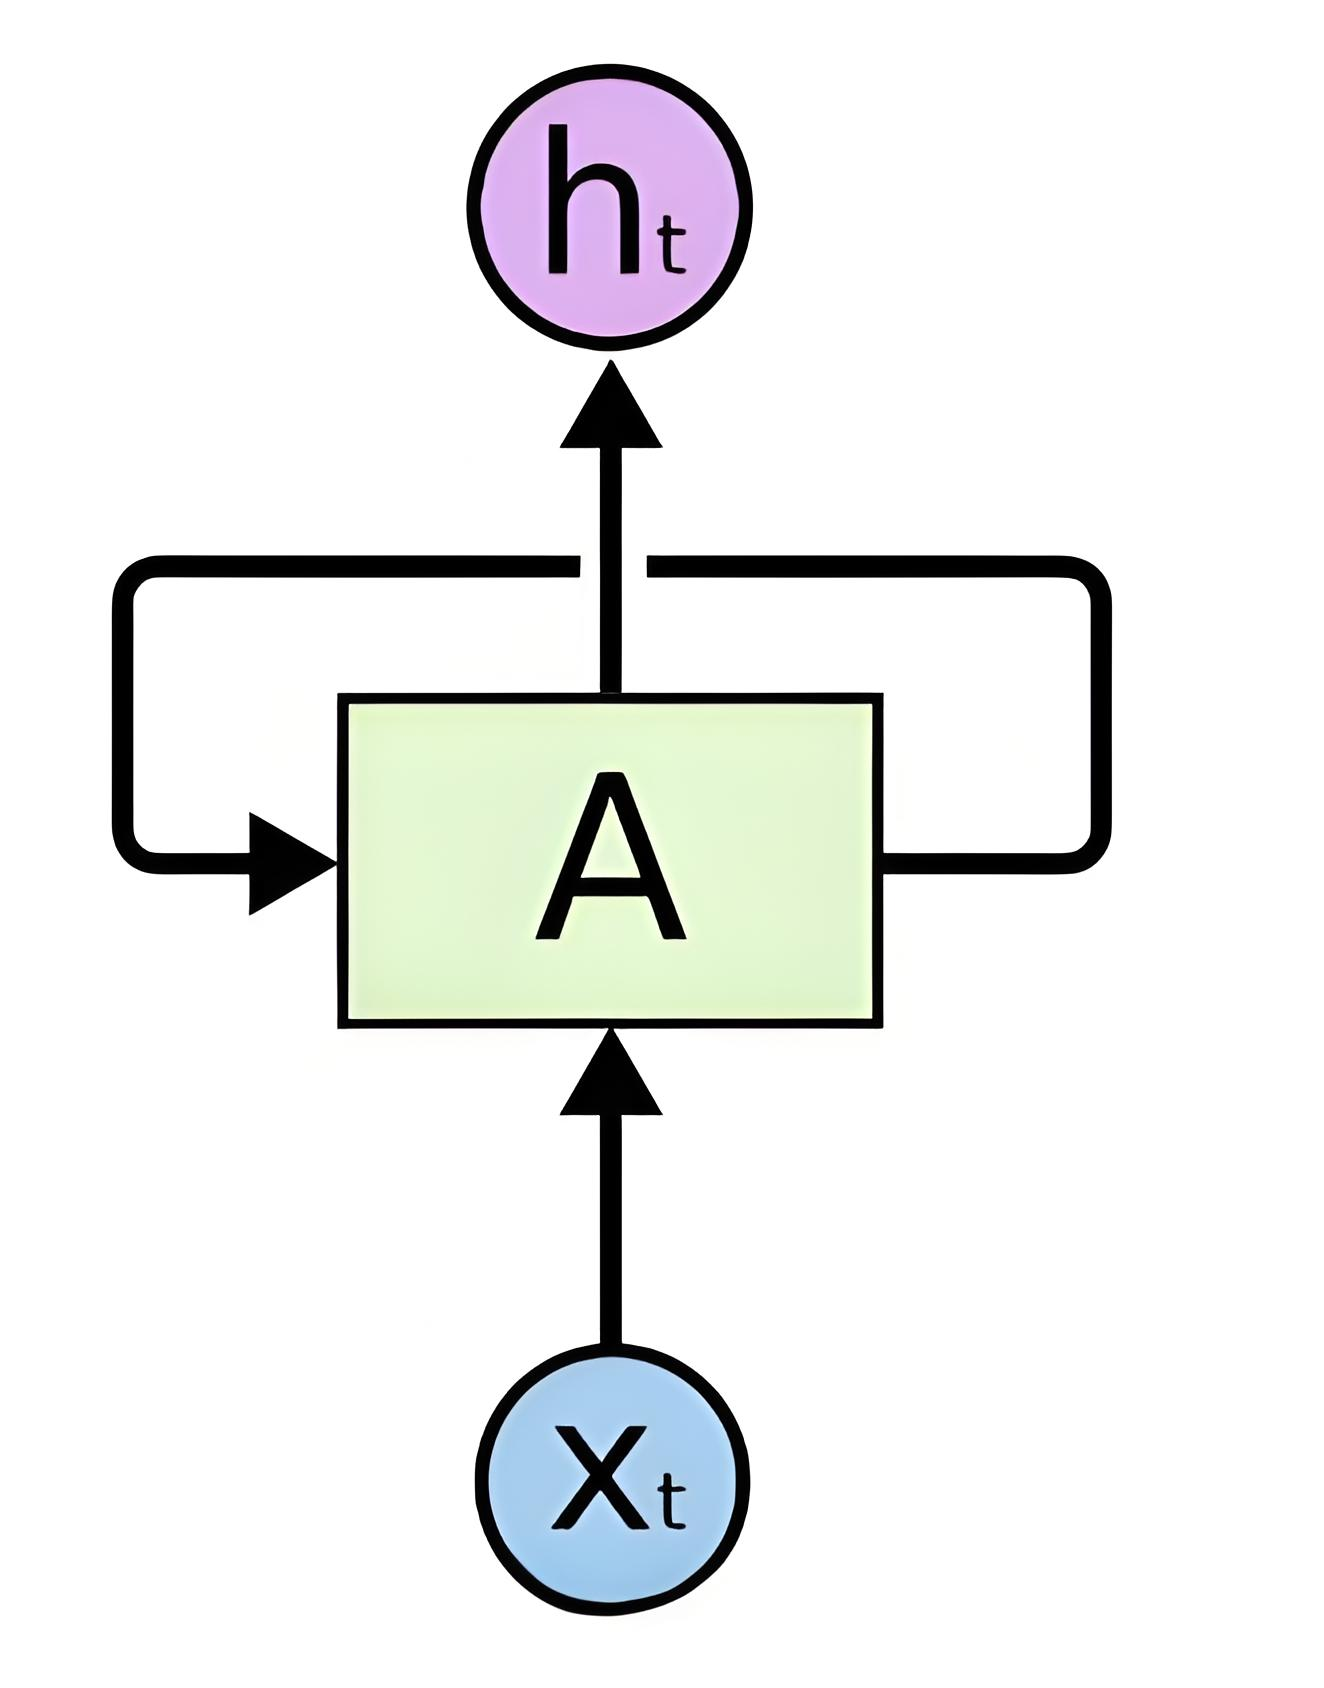
\includegraphics[width=0.2\linewidth]{../img/rnn.png}
      \caption{RNN Unit}
      \label{fig:rnn}
\end{figure}

However, due to the long average length of the samples in this project, using a conventional RNN will face the problem of gradient explosion/vanishing, struggling to capture long-term dependencies. So a modified version of RNN, known as Bidirectional Long Short-Term Memory (Bi-LSTM), is utilized in the project. It addresses the limitations of traditional RNN by adding specialized memory structures that can selectively retain and discard information over time, thus more effectively modeling long-term dependencies in textual data.

\subsection{Bi-LSTM}
\noindent
LSTM enhances the capabilities of traditional RNN by introducing specialized components like input gates, output gates, forget gates and cells. The structure of a LSTM unit is shown in Figure \ref{fig:lstm}. The process of updating the state of each LSTM unit is given below, assuming that the current time step is noted as $t$, and the tensor generated by the token at that position after word embedding is denoted as $X_t$.

\begin{figure}[h]
      \centering
      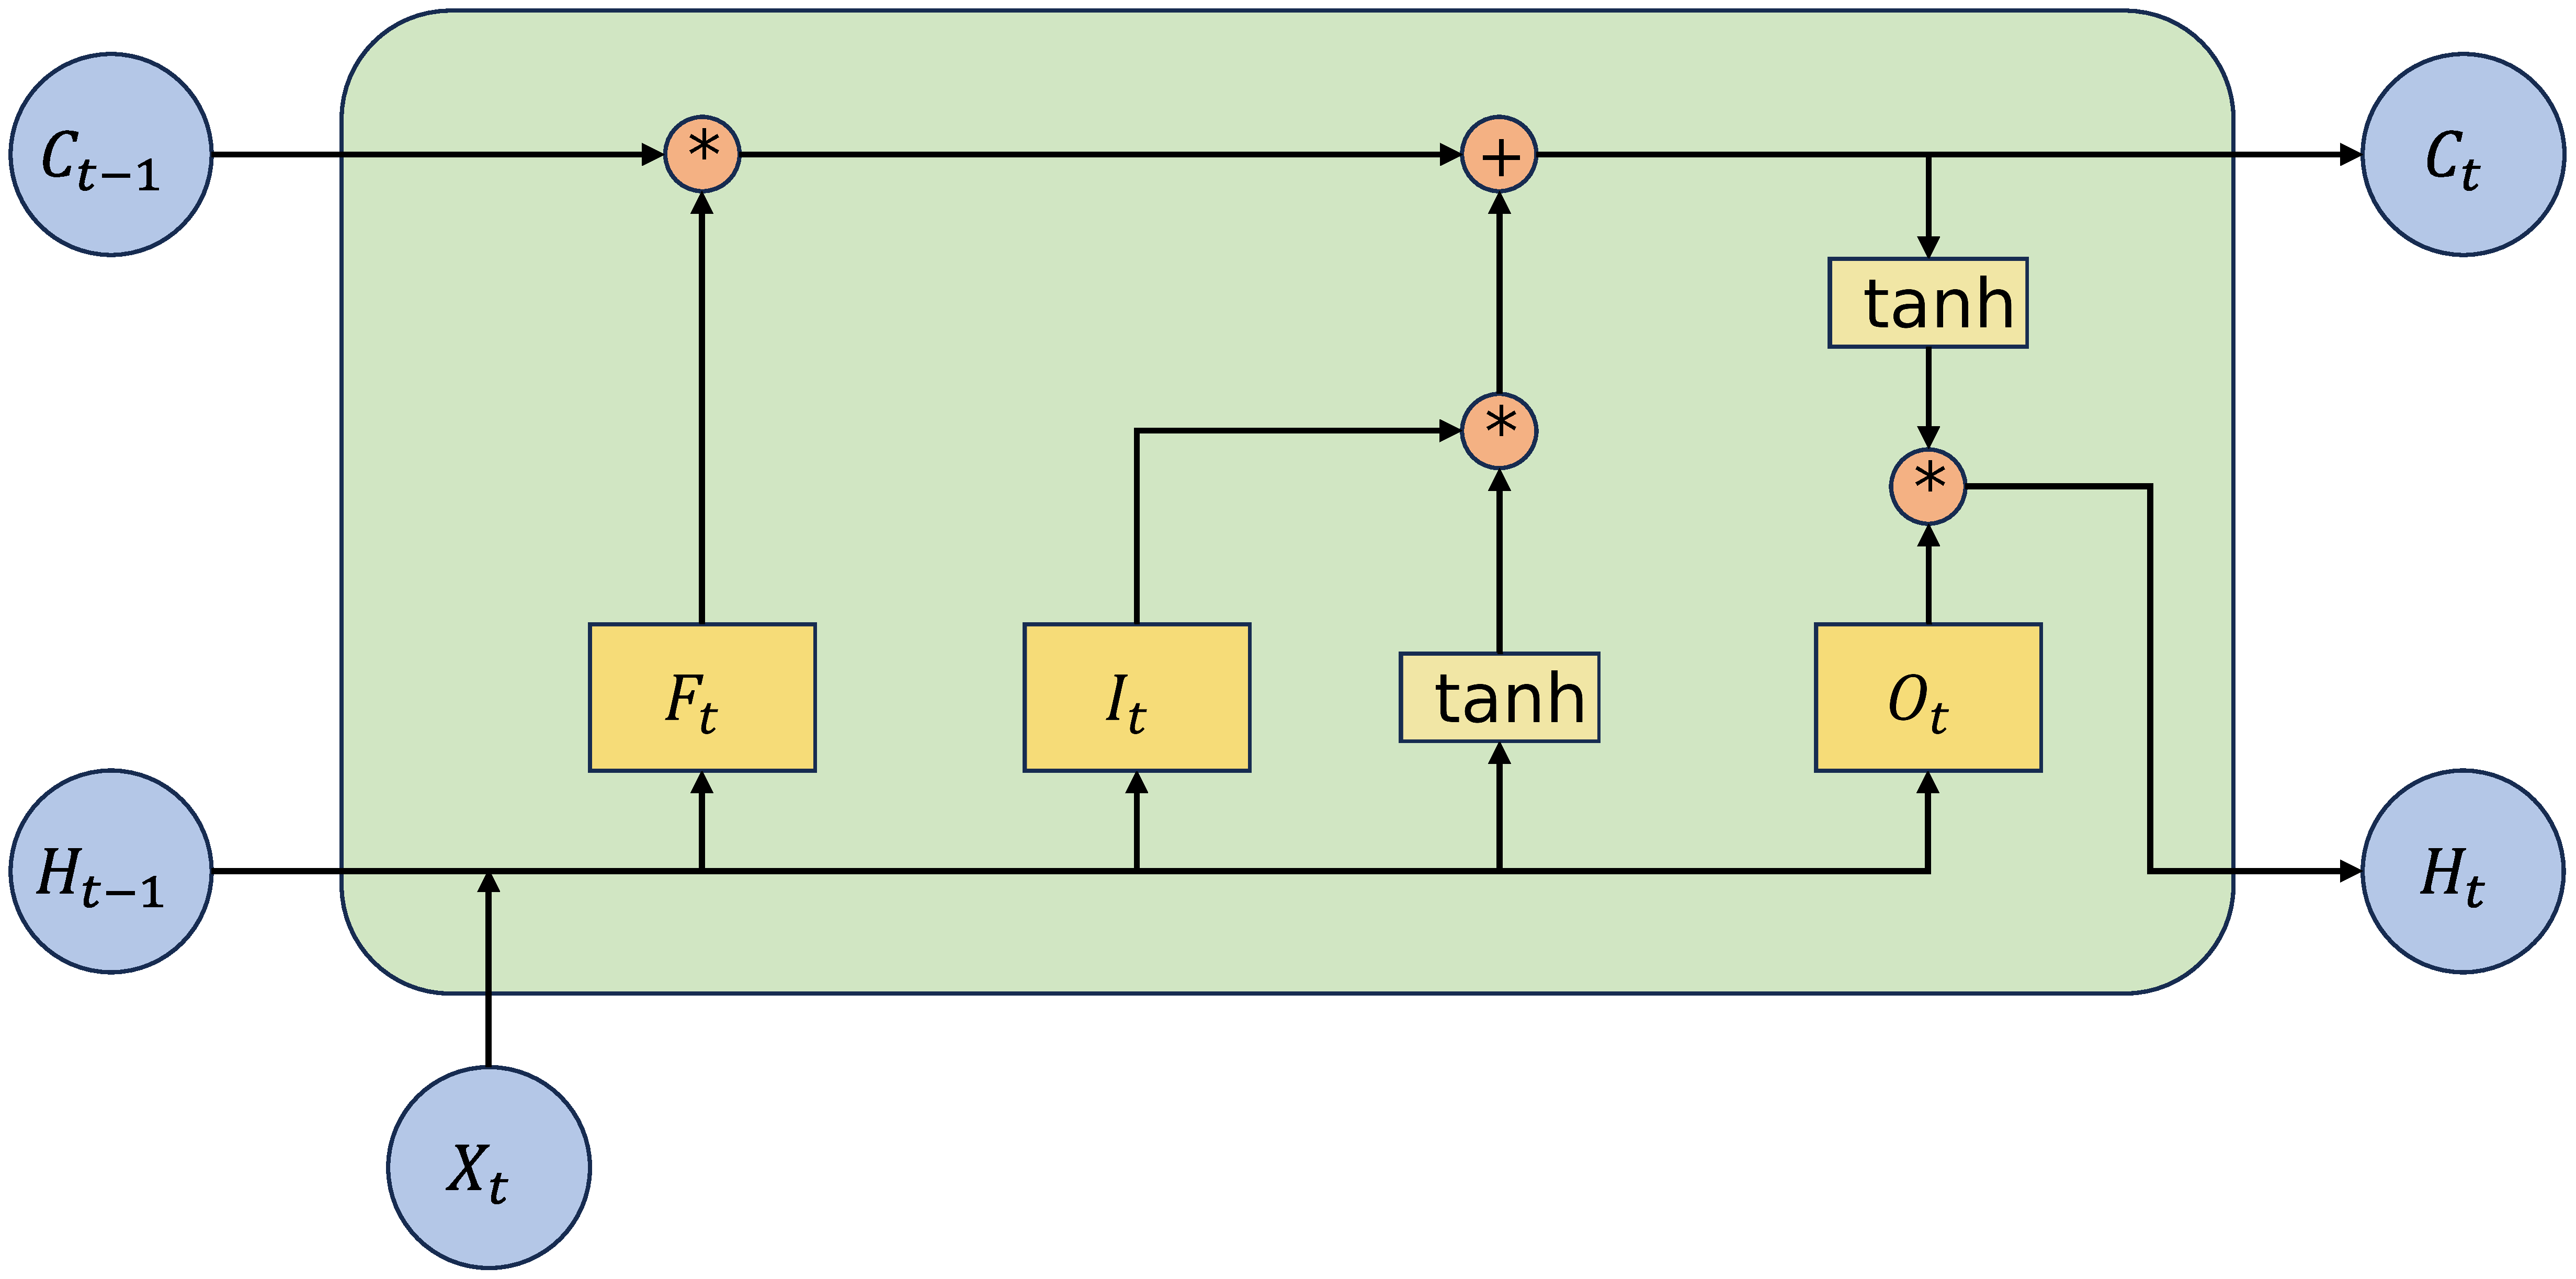
\includegraphics[width=0.7\linewidth]{../img/lstm.eps}
      \caption{LSTM Unit}
      \label{fig:lstm}
\end{figure}

The core of LSTM is the cell state, depicted as a horizontal line traversing the top of Figure \ref{fig:lstm}. The cell state acts like a conveyor belt, passing through all LSTM cells but with few branches to maintain information flows relatively unchanged. The output of information passed to the next unit is called a cell, noted as $C_t$.

The forget gate, noted as $F_t$, plays a crucial role in determining the extent to which information from the previous time step's cell should be retained in the current time step. In other words, it determines what information is irrelevant in determining whether the text contains suicidal ideation and decides what to discard from the previous cell state. The gate takes inputs from the previous hidden state $H_{t-1}$ and the current input $X_t$. After passing a sigmoid function, it outputs a vector, whose values range between $0$ and $1$. The value represents the importance of the information for identifying suicidal ideation, determining how much information can be retained. Multiplied element-wise with the corresponding element of the previous cell $C_{t-1}$, the information is partially discarded according to this value. The process of updating the forget gate is represented as follows:

\begin{eqnarray}
      F_t = \sigma(W_f\cdot[H_{t-1}, X_t] + b_f)
      \label{forgetgate}
\end{eqnarray}

The LSTM introduces an additional component known as the candidate memory cell $\tilde{C_t}$, representing the the proposed update to the cell state, obtained from the input data $X_t$ and the previous hidden state $H_{t-1}$ via an activation function. The activation function for updating the cell state is usually the hyperbolic tangent (tanh) function. The computation of $\tilde{C_t}$ is expressed as follows:

\begin{eqnarray}
      \tilde{C_t} = \tanh(W_C\cdot[H_{t-1}, X_t] + b_C)
      \label{ctilde}
\end{eqnarray}

The input gate $I_t$ is responsible for determining the proportion of the current time step's input to retain. It processes the input information for the current time step, which consists of two components: the hidden state $h_{t-1}$ and the input $X_t$. $I_t$ is used to control which features of $\tilde{C_t}$ are used to update $C_t$.

\begin{eqnarray}
      I_t = \sigma(W_i\cdot[H_{t-1}, X_t] + b_i)
      \label{inputgate}
\end{eqnarray}

The current cell state $C_t$ is updated by combining the suicidal memory inherited from the previous state and the new suicidal information selected by the input gate. The symbol "$\circ$" denotes the multiplication of the corresponding elements of two vectors.

\begin{eqnarray}
      C_t = F_t \circ C_{t-1} + I_t \circ \tilde{C_t}
      \label{ct}
\end{eqnarray}

The output gate $O_t$ determines which parts of the cell state will be output as the current hidden state $H_t$. The output gate takes into account the current input and previous hidden state, and outputs a value between $0$ and $1$ for each component of the cell state.

\begin{eqnarray}
      O_t = \sigma(W_o\cdot[H_{t-1}, X_t] + b_o)
      \label{outputgate}
\end{eqnarray}

Meanwhile, the cell state is processed through tanh to get a value between $-1$ and $1$, effectively normalizing the output. The output of the sigmoid gate, representing the filter function, is then multiplied element-wise with the processed cell state to obtain the hidden state $H_t$. This step ensures that only information relevant to the judgement of suicidal ideation, as determined by the output gate, is retained and passed on to the next time step. The process is represented as follows:

\begin{eqnarray}
      H_t = O_t \circ \tanh(C_t)
      \label{ht}
\end{eqnarray}

When multiple LSTM units are connected in sequence, a unidirectional LSTM layer is formed. The cell at time step $t$ captures the context leading up to that point. Although processing input sequence from start to end can extract forward associations between words, and it is also consistent with human reading habits, natural language is inherently very complex. Later parts of the content may also provide interpretations for the earlier words, which means that both forward and backward contextual may influence whether the word expresses suicidal ideation. 

To address this, a bidirectional LSTM (Bi-LSTM) architecture is employed, integrating both forward and backward information processing capabilities. The forward-direction LSTM layer optains the incluence of the preceding texts on whether the current word contains suicidal ideation, with a reverse-direction LSTM layer processing the same text in the reverse order to capture the impact of latter texts. By combining suicidal information from both directions, the Bi-LSTM network improves its ability to understand and interpret the nature language, making it a more robust model for NLP tasks. The structure of Bi-LSTM layer is shown in the Figure \ref{fig:bilstm}.

\begin{figure}[h]
      \centering
      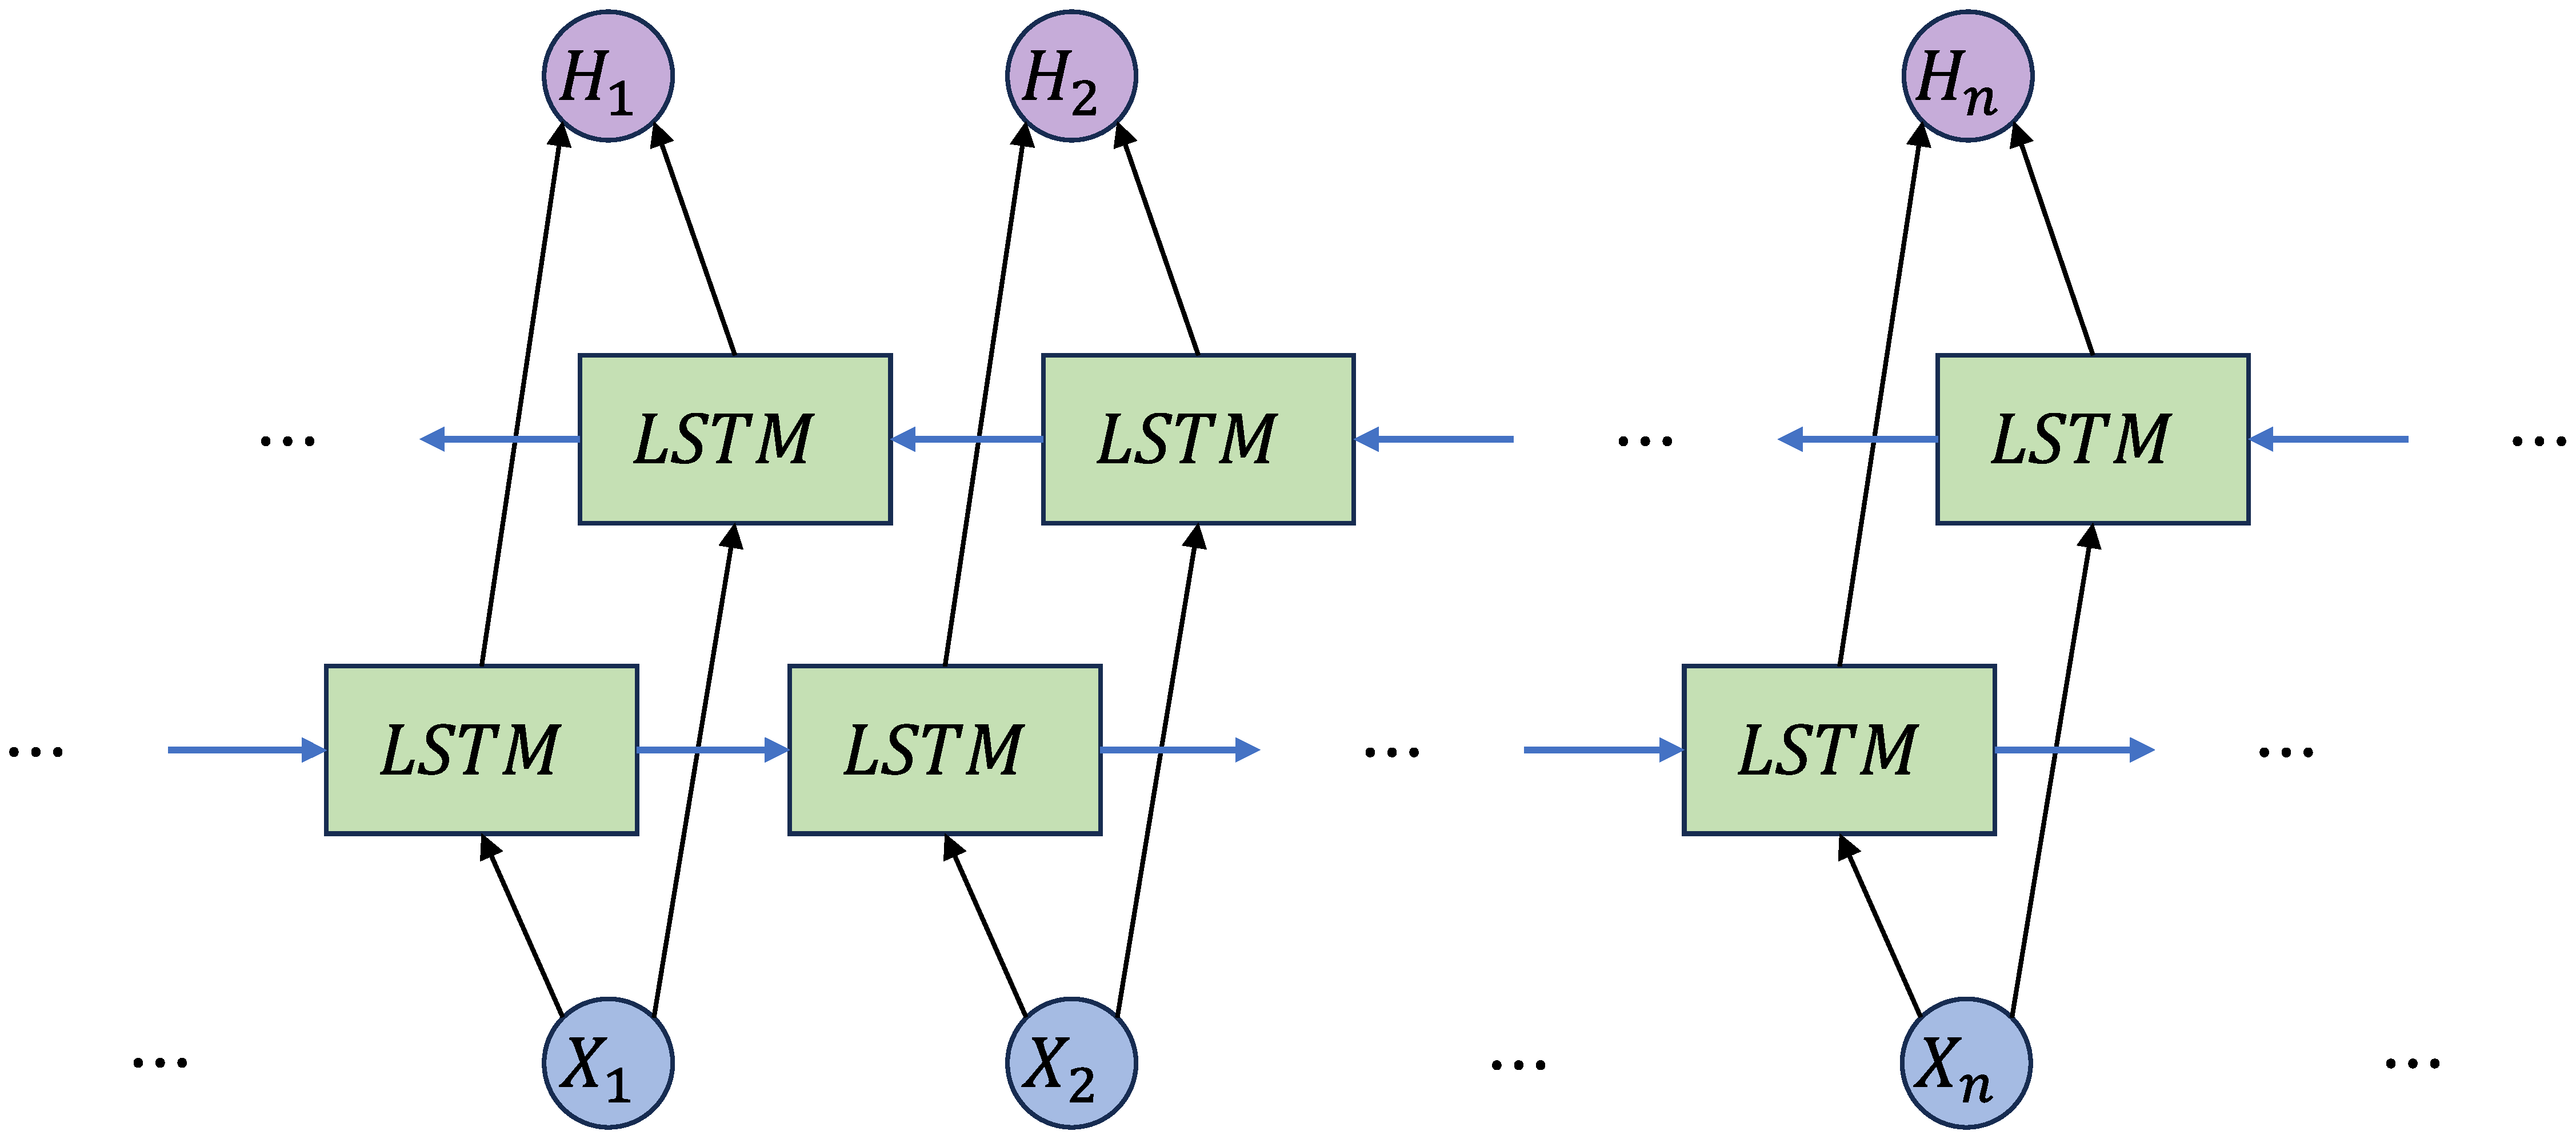
\includegraphics[width=0.7\linewidth]{../img/bilstm.eps}
      \caption{Bi-LSTM Layer}
      \label{fig:bilstm}
\end{figure}

\subsection{Building Bi-LSTM Model}
\noindent
A basic neural network consists of an embedding layer, a hidden layer, and a fully connected layer. In this project, the BiLSTM network includes essential components: a word embedding layer, a hidden layer, a dropout layer, a fully connected layer, and a classification layer. The output of each layer serves as the input of the subsequent layer, allowing the model to capture the semantics and make accurate predictions about whether the sentence contains suicidal ideation or not.

Embedding Layer: This layer converts input words into dense vector representations, capturing semantic information. To maintain consistency with the embedding technique employed before, the bert embedding layer is still used here as the embedding layer in the model. Each word will be transformed into a 768-dimensional vector, serving as input to the subsequent hidden layer.

Hidden Layer: The hidden layer does not receive signals directly from the outside world, nor does it transmit signals directly to the outside world. Its role is to process the input data and extract the features of the data to help the network better recognize suicidal ideation in text. In this model, the BiLSTM layer acts as the hidden layer to extract features of suicide ideation from the data.

Dropout Layer: Dropout technique\cite{srivastava2014dropout} is a regularisation technique, aimed at reducing overfitting by randomly discarding the information in certain neurons in the previous layer according to a certain proportion during the training process. But the overuse of dropout may result in some information affecting the judgement of suicidal ideation being discarded, which will influence the accuracy of the model.

Fully Connected Layer: In traditional neural networks, fully connected layer is a linear layer whose output is a linear combination of the inputs along with a bias. In deep learning, it is typically employed to convert high-dimensional data into low-dimensional data for classification or regression. In this project, the output of this layer is a 2-dimensional vector indicating the degree to which the sentence is predicted as suicide or nun-suicide respectively.

Classification Layer: The final layer of the network, here a sigmoid layer, outputs the probability distribution over the possible classes. It outputs two probability scores indicating the likelihood that the model considers the input to be suicidal and non-suicidal separately.

\subsection{Bi-LSTM Model Performance}
\noindent
In this project, the model is trained with mini-batch.The cross-entropy loss function is chosen as the loss function, and the Adam optimiser is used for optimisation. Adam optimizer, introduced by Kingma and Ba\cite{kingma2014adam}, stands as one of the most widely used optimisation algorithm at present.

There are many hyperparameters that need to be determined manually when constructing the network, so the choice of parameters has a different impact on the performance of the model. In order to get the best results from the model, a stratified 5-fold cross-validation is used to train and validate the different hidden layer output dimensions (hidden\_size), number of hidden layers (num\_layers), and learning rate (learn\_rate) respectively, so as to obtain the parameter combination with the best validation results. F1 score is chosen as the metric for evaluating the model performance, and Figure \ref{fig:tune} illustrates the performance of the model for different combinations of hyperparameters.

\begin{figure}[h]
      \centering
      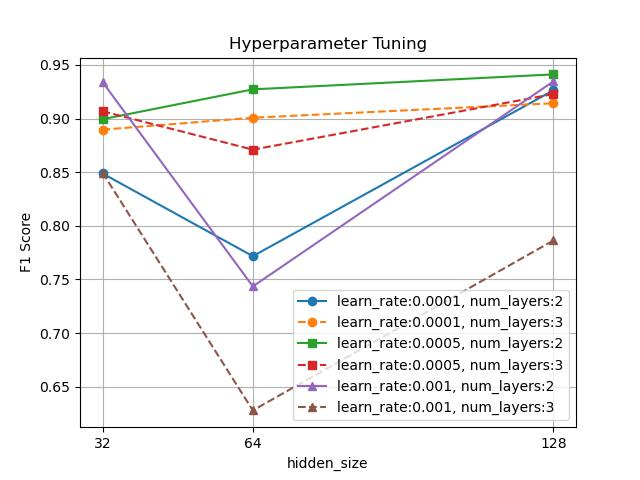
\includegraphics[width=0.8\linewidth]{../img/lstm_tuning.jpg}
      \caption{Hyperparameter Tuning}
      \label{fig:tune}
\end{figure}

It is simple to determine that the model has the highest F1 score when the hidden layer output dimension is 128, the number of hidden layers is taken to be 2 and the learning rate is 0.0005. Table \ref{tab:tuning} shows the specific performance metrics of the model under different combinations, where the best performing values for each metric are bolded. When the combination of hyperparameters with the highest F1 scores is utilized, the model outperforms other combinations in both Accuracy and Recall. Based on the results of the above comparisons, the final parameter selection is detailed in the Table \ref{tab:lstmhyperparameter}. 

\begin{table}[h]
      \centering
      \begin{tabular}{ccc|cccc}
            \hline
            learning\_rate & num\_layers & hidden\_size & Acc (\%) & Pre (\%) & Rec (\%) & F1 (\%) \\
            \hline
            \multirow{6}*{0.0001} & \multirow{3}*{2} & 32  & 85.38 & 87.65 & 82.44 & 84.88 \\
                                  &                  & 64  & 84.04 & 91.39 & 74.86 & 77.17 \\
                                  &                  & 128 & 92.59 & 92.24 & 93.16 & 92.64 \\
            \cline{3-7}
                                  & \multirow{3}*{3} & 32  & 88.98 & 89.06 & 88.94 & 88.97 \\
                                  &                  & 64  & 90.32 & 91.78 & 88.63 & 90.08 \\
                                  &                  & 128 & 91.58 & 92.90 & 90.28 & 91.43 \\
            \cline{2-7}
            \multirow{6}*{0.0005} & \multirow{3}*{2} & 32  & 89.90 & 89.29 & 90.75 & 89.94 \\
                                  &                  & 64  & 92.78 & 93.50 & 92.09 & 92.73 \\
                                  &                  & 128 & \textbf{94.07} & 93.36 & \textbf{94.94} & \textbf{94.12} \\
            \cline{3-7}
                                  & \multirow{3}*{3} & 32  & 90.95 & 91.60 & 90.55 & 90.69 \\
                                  &                  & 64  & 87.87 & 91.53 & 83.58 & 87.10 \\
                                  &                  & 128 & 92.41 & 94.12 & 90.63 & 92.29 \\
            \cline{2-7}
            \multirow{6}*{0.001}  & \multirow{3}*{2} & 32  & 93.41 & 93.26 & 93.57 & 93.41 \\
                                  &                  & 64  & 81.20 & 87.94 & 72.58 & 74.35 \\
                                  &                  & 128 & 93.64 & \textbf{95.69} & 91.42 & 93.48 \\
            \cline{3-7}
                                  & \multirow{3}*{3} & 32  & 85.26 & 86.31 & 83.85 & 84.96 \\
                                  &                  & 64  & 76.54 & 90.57 & 58.75 & 62.78 \\
                                  &                  & 128 & 85.51 & 92.25 & 76.94 & 78.63 \\
            \hline
      \end{tabular}
      \caption{Cross-Validation Results for Various Hyperparameter Combinations}
      \label{tab:tuning}
\end{table}

\begin{table}[h]
      \centering
      \begin{tabular}{cc}
            \hline
            Hyperparameter & Value \\
            \hline
            embedding\_size & 768    \\
            hidden\_size    & 128    \\
            num\_layers     & 2      \\
            num\_classes    & 2      \\
            learning\_rate  & 0.0005 \\
            epochs          & 4      \\
            \hline
      \end{tabular}
      \caption{Hyperparameter Settings for Bi-LSTM}
      \label{tab:lstmhyperparameter}
\end{table}

\begin{figure}[!h]
      \centering
      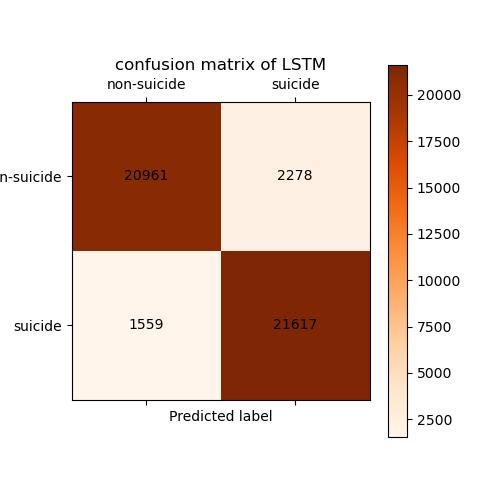
\includegraphics[width=0.4\linewidth]{../img/cm_LSTM.jpg}
      \caption{Confusion Matrix of Bi-LSTM}
      \label{fig:cm_LSTM}
\end{figure}

After the model being trained on the training set, Figure \ref{fig:cm_LSTM} shows the confusion matrix on the test set. In order to demonstrate the effectiveness of the Bi-LSTM model on word embedding, comparison experiments are employed. The performance of the baseline model, which also utilized bert embedding, is compared with the current model on the same test set.

Figure \ref{fig:rocLRLSTM} shows the ROC curves of the two models. It can be seen that the area under the curve of the Bi-LSTM model is significantly larger than that of the LR model, indicating that the comprehensive performance of Bi-LSTM is better than that of LR. The results in Table \ref{tab:lstmmetrics} demonstrate the specific performance comparison between the two models when the threshold is 0.5. The scores of Bi-LSTM are much higher than those of LR in all the four metrics.

This observation provides strong evidence that Bi-LSTM is able to fully learn the contextual information extracted from word embedding, and is able to mine more details of suicidal tendencies in the text than LR, resulting in a better performance.

\begin{table}[!h]
      \centering
      \begin{tabular}{c|cccc}
            \hline
            Model & Acc(\%) & Pre(\%) & Rec(\%) & F1(\%) \\
            \hline
            LR      & 73.66 & 75.63 & 69.88 & 72.64 \\
            Bi-LSTM & 94.79 & 93.66 & 96.09 & 94.86 \\
            \hline
      \end{tabular}
      \caption{Performance Mertics of Bi-LSTM and Baseline Model}
      \label{tab:lstmmetrics}
\end{table}

\begin{figure}[h]
      \centering
      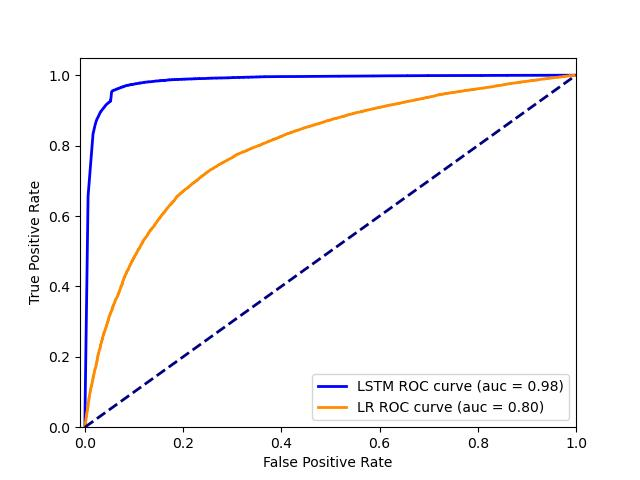
\includegraphics[width=0.48\linewidth]{../img/roc_LRb&LSTM.jpg}
      \caption{ROC Curves of Bi-LSTM and Baseline Model}
      \label{fig:rocLRLSTM}
\end{figure}

\subsection{Bi-LSTM Model Explanation}
\noindent
To interpret the predicted results of the model, SHAP is used as an explainer. Here the wrongly predicted examples have been selected, trying to explain the reason behind such errors through SHAP. Figure \ref{fig:lstmshap}\ref{sub@lstm_fp} shows a sample where the Bi-LSTM model misclassified a non-suicidal category as a suicidal one, and Figure \ref{fig:lstmshap}\ref{sub@lstm_fn} shows a suicide category example being judged as non-suicide.

\begin{figure}[h]
      \centering
      \subfloat[False Positive Sample]{
            
\includegraphics[width=0.9\linewidth]{../img/lstm_fp.png}
            \label{lstm_fp}}
      \hfil
      \subfloat[False Negative Sample]{
            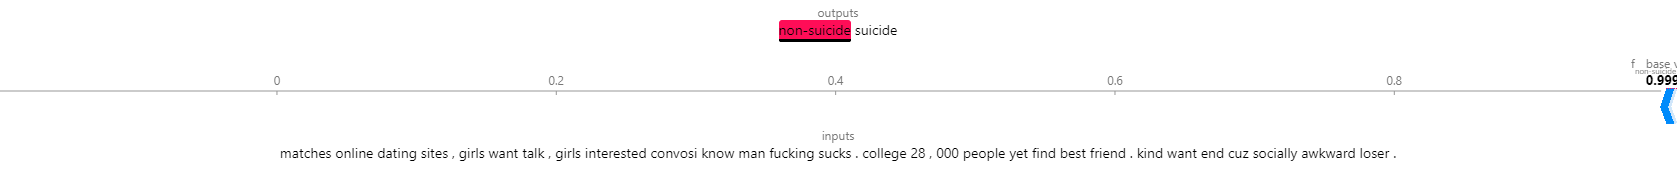
\includegraphics[width=0.9\linewidth]{../img/lstm_fn.png}
            \label{lstm_fn}}
      \caption{Wrongly Predicted Samples Explained by SHAP}
      \label{fig:lstmshap}
\end{figure}

It can be found that the Bi-LSTM model treats the words 'ending' and 'life' as strong suicidal tendencies, interpreting them as indicative of strong suicidal tendencies, thus significantly impacting the prediction outcome. However, the original text can be seen to be just a person's complaint about the loss of the game, thus leading to an error in the model's prediction. In the other sentence, it is not clear which word plays a significant influence on the model's prediction. It also reveals that the shapley value can aid in understanding the reason behind the model's decision to a certain extent, and can't entirely explain the prediction process.

\section{Large Language Model}
\noindent
LSTM has been able to have superior performance in this task by considering information of contextual temporal order. However, as new techniques continue to emerge, large language models are offering even better results and are gradually becoming dominant in the NLP field. In this context, an attempt is made to further enhance the task performance by utilizing the current mainstream BERT model.

\subsection{BERT}
\noindent
BERT, proposed by Google in 2018\cite{devlin2018bert}, is a pre-trained language model that represents a significant advancement in NLP. It is a bidirectional pre-training model that comprehensively understands the context and the relationship between words from both left and right side, and can therefore process natural language with remarkable accuracy.

The structure of the BERT network is shown in Figure \ref{fig:bertstructure}. It mainly consists of multiple Transformers encoders, applying unsupervised pre-training on a large amount of data, and then can be fine-tuned for different NLP tasks. The Transformers network employs self-attention to calculate the influence of each word in a sentence on every other word, or by recording an "attention score". It allows for superior encoding or decoding of sequential data, leading to enhanced performance in multiple tasks. Figure \ref{fig:transformerstructure} shows the structure of the Transformers network. The left part of this is the encoder of Transformers, which is used as the base structure of the BERT model.

\begin{figure}[h]
      \centering
      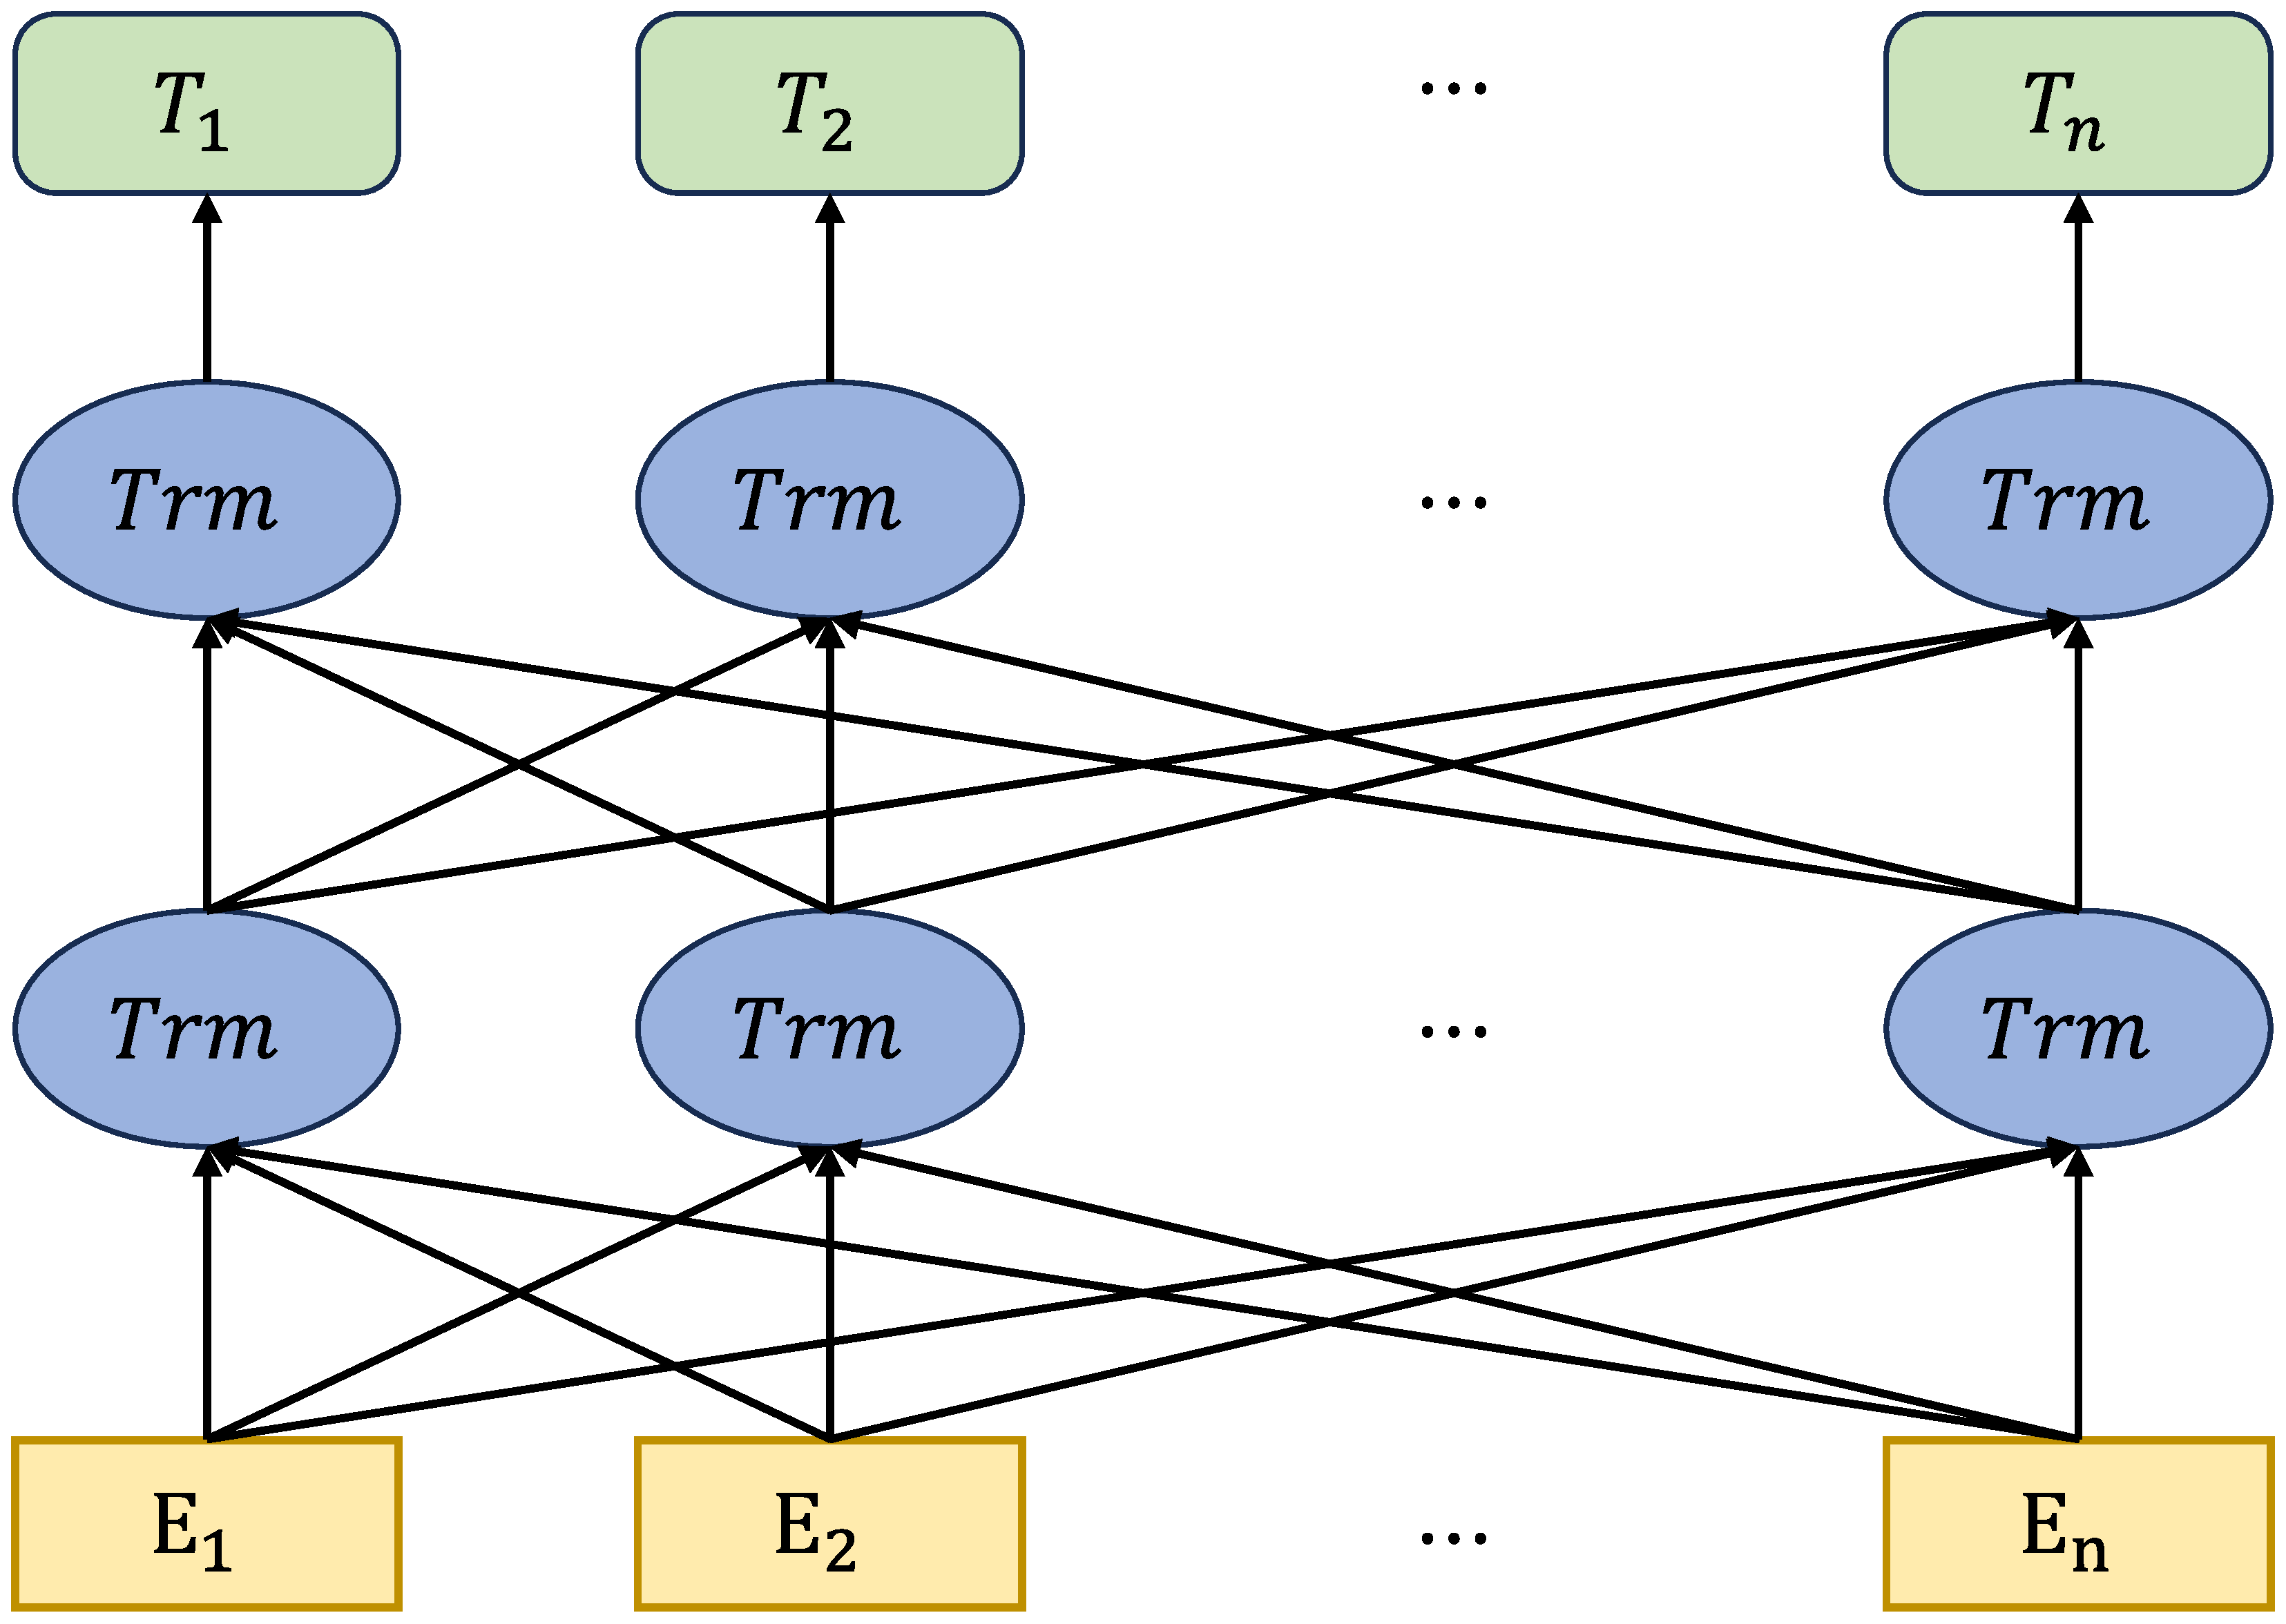
\includegraphics[width=0.4\linewidth]{../img/bert.eps}
      \caption[BERT Pre-training Language Model Diagram]{BERT Pre-training Language Model\cite{devlin2018bert}}
      \label{fig:bertstructure}
\end{figure}

\begin{figure}[h]
      \centering
      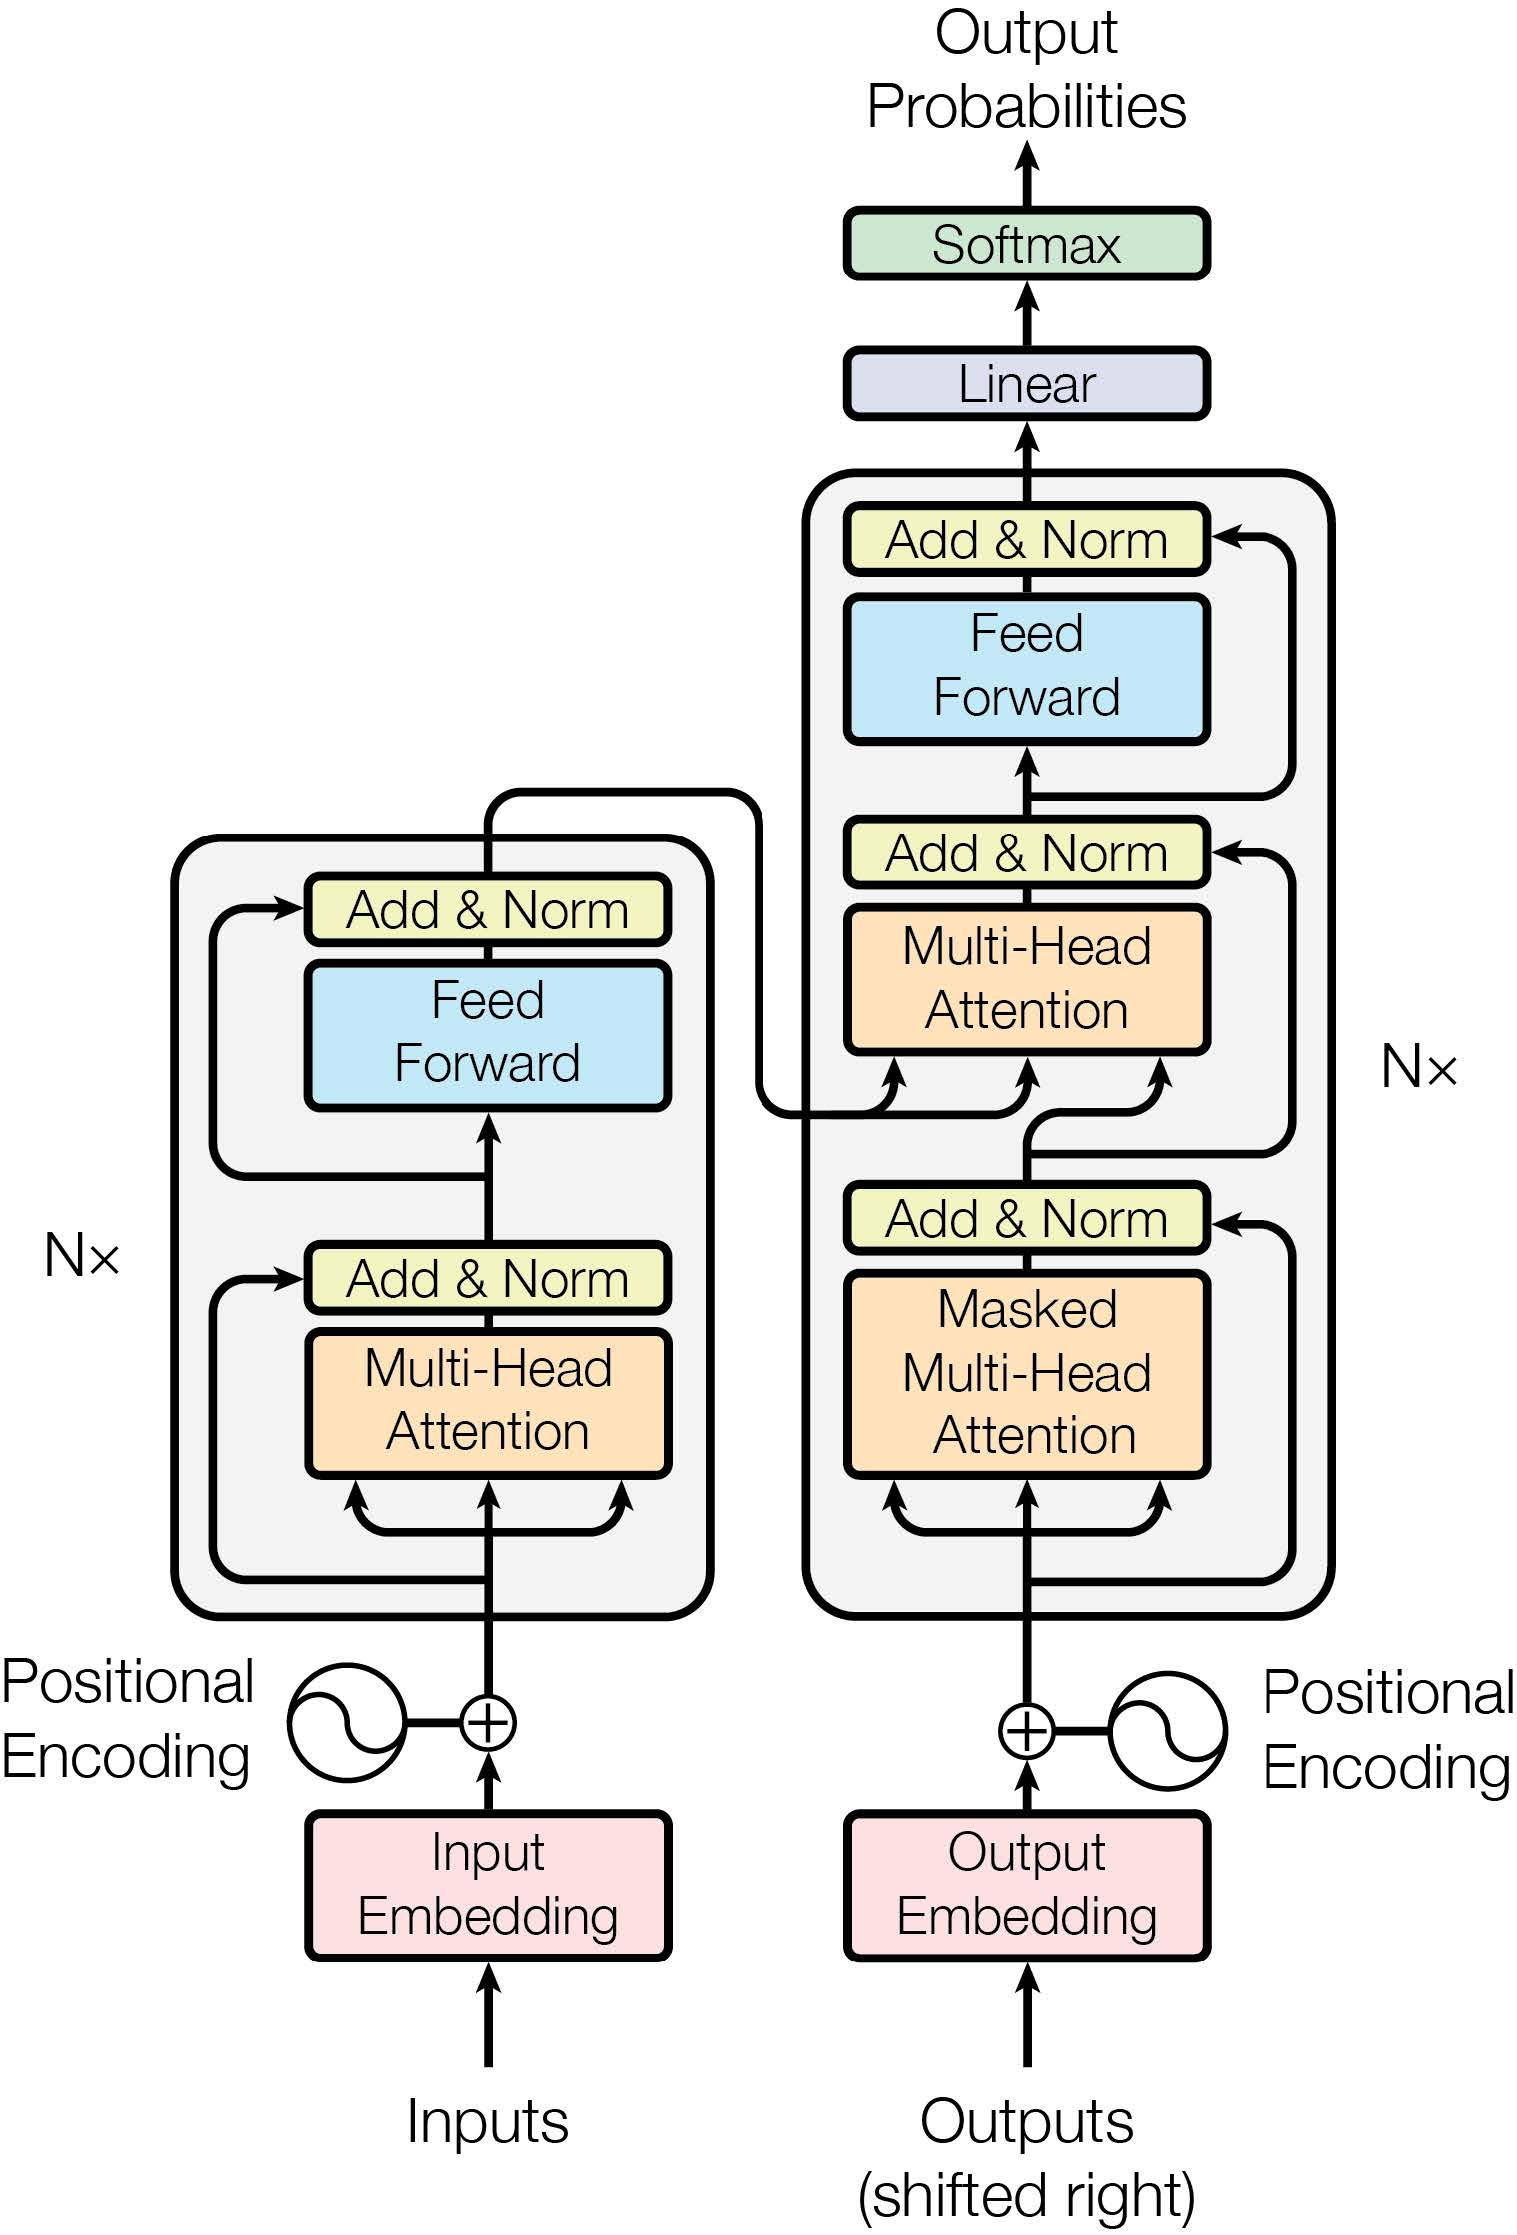
\includegraphics[width=0.5\linewidth]{../img/transformer.jpg}
      \caption[Transformers Network Structure]{Transformers Network Structure\cite{vaswani2017attention}}
      \label{fig:transformerstructure}
\end{figure}

The training of the BERT model involves two key phases: pre-training and fine-tuning. In the pre-training phase, the BERT model introduces a Masked Language Model (MLM) task and a Next Sentence Prediction (NSP) task. 

In the MLM task, 15\% of the words in the training set are randomly replaced with [MASK] token, and the replaced words are predicted based on known contextual information. The masked words have an 80\% probability of being directly replaced with [MASK] token, a 10\% probability of being replaced with other words, and a 10\% probability of retaining the original words unchanged. 

In the NSP task, BERT randomly replaces some sentences in order to learn the relationship between sentences pairs. It then predicts whether the second sentence follows the first sentence in the original text or not. This task helps BERT understand the contextual relationships between consecutive sentences. After the model is obtained through pre-training, it can then be fine-tuned to provide better performance for downstream tasks.

\subsection{BERT Downstream Tasks}
\noindent
Without changing the internal structure of the BERT model, various NLP tasks can be achieved by adding task-specific networks after the encoding layer. The task of this project is to identify the suicide ideation, and the fine-tuned approach is shown in Figure \ref{fig:bfsc}. 

\begin{figure}[h]
      \centering
      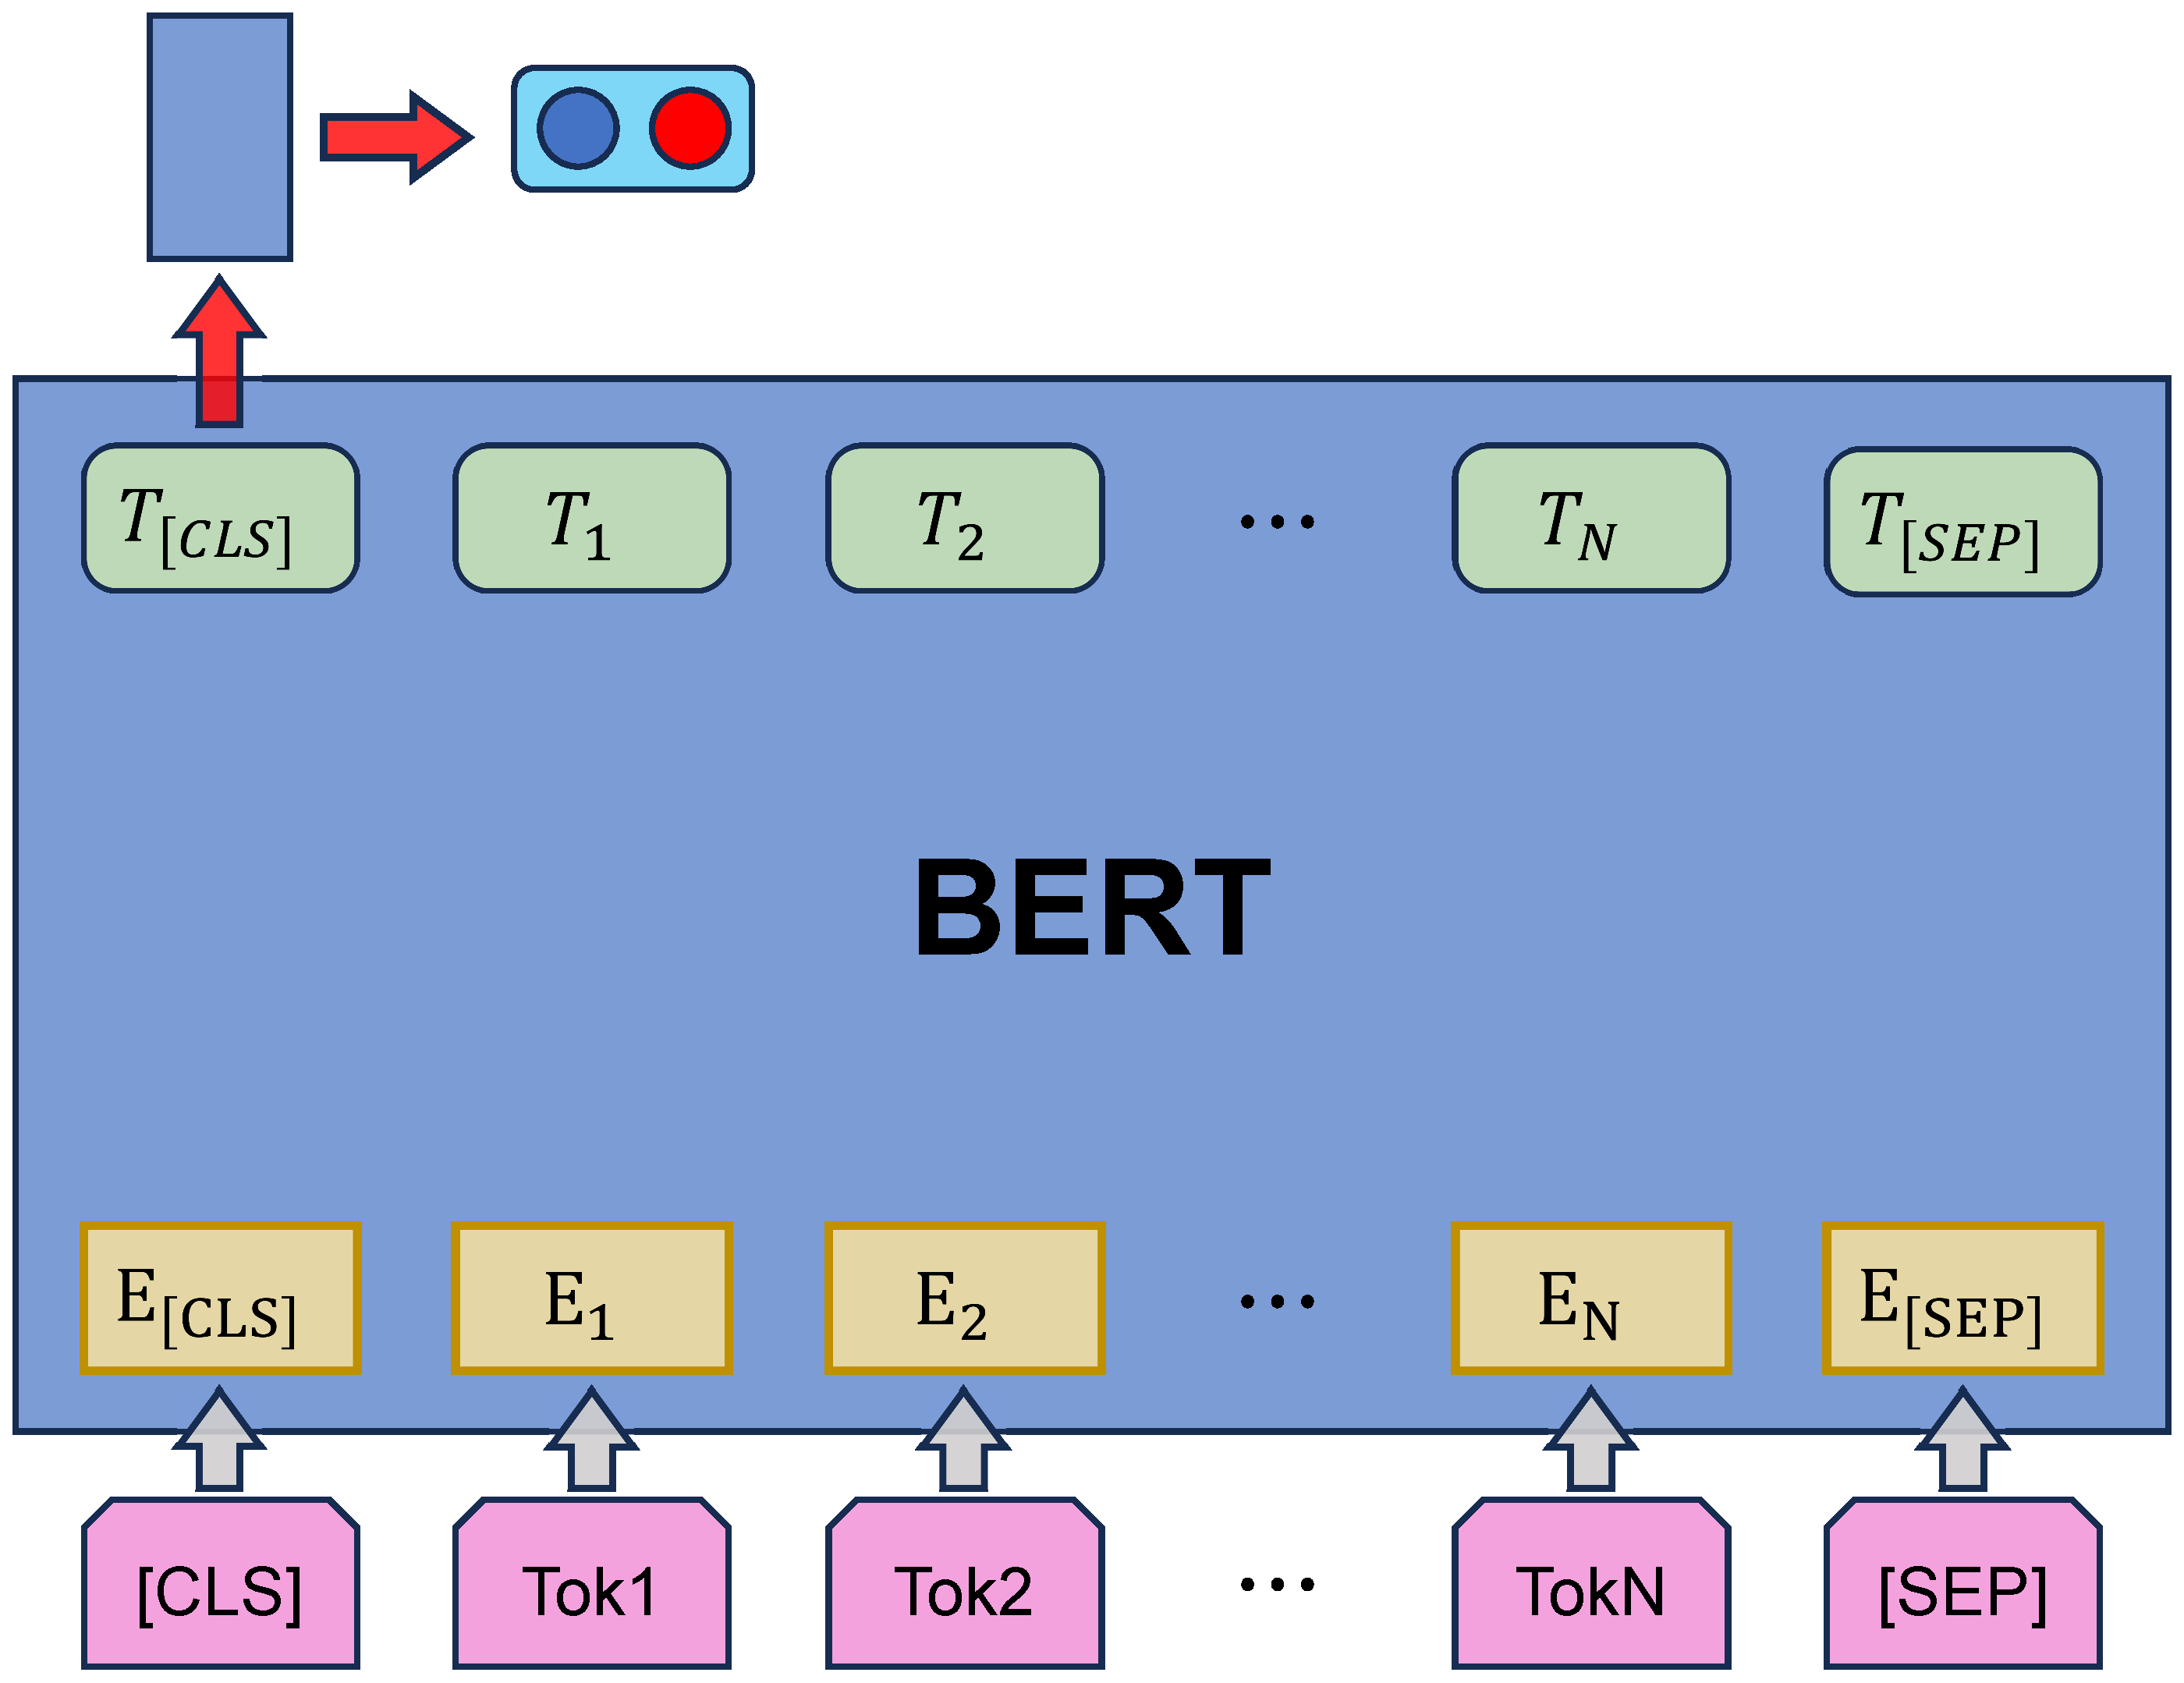
\includegraphics[width=0.5\linewidth]{../img/bfsc.eps}
      \caption{Fine-Tuning for Single Sentence Classification}
      \label{fig:bfsc}
\end{figure}

The BERT model inserts a [CLS] token at the beginning of the input text, shown in Figure \ref{fig:bert_embedding}, and utilizes the output vector corresponding to this token as a semantic representation of the whole text. Unlike other tokens, the [CLS] token has no inherent semantics, allowing it to integrate information from all tokens in the sentence more fairly. Therefore the output of this token is usually used for sentence classification tasks.

An additional output layer is appended to map the output 768-dimensional vectors into the final classification space. In this project, the 768-dimensional vector is mapped into a 2-dimensional vector space, and a softmax layer is utilized to generate the final result of sentiment classification, indicating the likelihood of being a "suicide" sample.

During the fine-tuning process, the model is trained on a specific dataset to enhance the capability to accurately identify whether a text contains suicidal ideation. Since the parameters have already been trained on a large-scale corpus during the pre-training process, which itself can do some semantic extraction, the training process can be faster and more accurate.

\subsection{BERT Model Performance}
\noindent
The AdamW optimizer\cite{loshchilov2019decoupled} is utilized in the process of training BERT model. AdamW is a variant of the Adam optimizer that distinguishes weight decay from the gradient update. This differentiation is based on the observation that the formulation of weight decay differs when applied to SGD and Adam. During training, most hyperparameters of the AdamW optimizer were kept at their default values. Only two were modified: "lr" for the learning rate and "eps" for the epsilon value that prevents division by zero in the optimizer. The hyperparameter settings of the experiment are shown in Table \ref{tab:berthyperparameter}:

\begin{table}[h]
      \centering
      \begin{tabular}{cc}
            \hline
            Hyperparameter & Value \\
            \hline
            num\_labels & 2      \\
            lr          & 5e-5   \\
            eps         & 1e-8   \\
            epochs      & 4      \\
            \hline
      \end{tabular}
      \caption{Hyperparameter Settings for BERT}
      \label{tab:berthyperparameter}
\end{table}

Figure \ref{fig:cm_BERT} shows the confusion matrix of the model. In order to compare whether the BERT model has better performance than the Bi-LSTM model, the performance metrics of the two models on the test set were put together for comparison. Figure \ref{fig:rocLSTMBERT} exhibits the ROC curves of both model, and Table \ref{tab:bertmetrics} shows the four performance metrics of the two models on the test dataset. 

\begin{figure}[h]
      \centering
      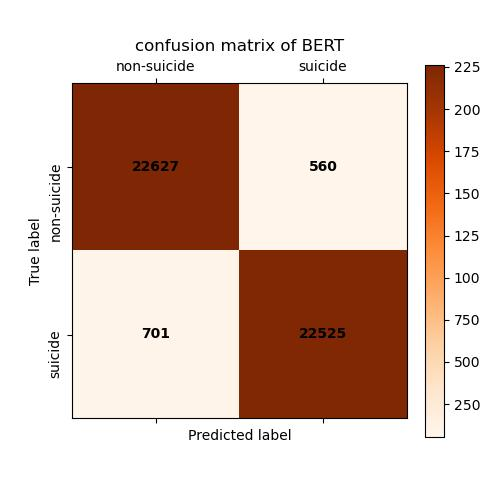
\includegraphics[width=0.46\linewidth]{../img/cm_BERT.jpg}
      \caption{Confusion Matrix of BERT}
      \label{fig:cm_BERT}
\end{figure}

\begin{figure}[!h]
      \centering
      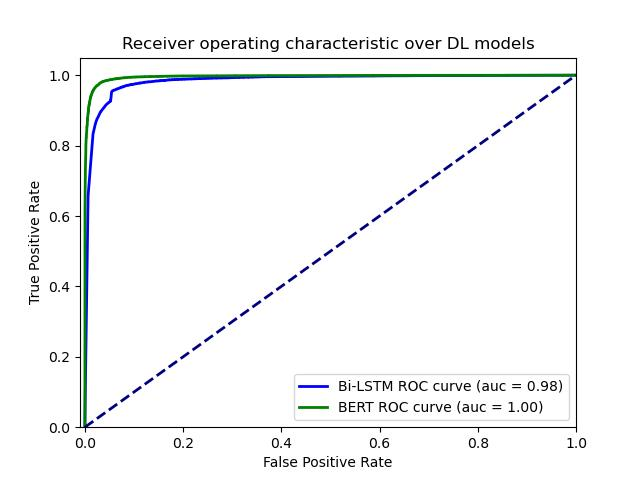
\includegraphics[width=0.5\linewidth]{../img/roc_BERT&LSTM.jpg}
      \caption{ROC Curves of BERT and Bi-LSTM}
      \label{fig:rocLSTMBERT}
\end{figure}

\begin{table}[!h]
      \centering
      \begin{tabular}{c|cccc}
            \hline
            Model & Acc(\%) & Pre(\%) & Rec(\%) & F1(\%) \\
            \hline
            Bi-LSTM & 94.79 & 93.66 & 96.09 & 94.86 \\
            BERT    & 97.28 & 97.57 & 97.00 & 97.28 \\
            \hline
      \end{tabular}
      \caption{Performance Mertics of BERT and Bi-LSTM}
      \label{tab:bertmetrics}
\end{table}

Conducting testing on both Bi-LSTM and BERT model, it is found that the BERT model outperforms the Bi-LSTM model in terms of accuracy, precision, recall, and F1 score. The BERT model exhibited superior performance across all metrics, indicating its effectiveness in accurately predicting suicide ideation in text. This comparison highlights the advantages of pre-trained language models like BERT, which can capture semantic relationships effectively. Consequently, the BERT model is selected as the preferred choice for deployment in real-world applications due to its superior performance and robustness in sentiment classification tasks.

\subsection{BERT Model Explanation}
\noindent
SHAP was likewise used to interpret the predictions of the BERT model. Samples that were wrongly predicted by the BERT model were also selected to analyse why the BERT model made wrong predictions respectively. Figure \ref{fig:bertshap} show the results of SHAP's explanations respectively.

\begin{figure}[h]
      \centering
      \subfloat[False Positive Sample]{
            
\includegraphics[width=0.9\linewidth]{../img/bert_fp.png}
            \label{bert_fp}}
      \hfil
      \subfloat[False Negative Sample]{
            
\includegraphics[width=0.9\linewidth]{../img/bert_fn.png}
            \label{bert_fn}}
      \caption{Wrongly Predicted Samples Explained by SHAP}
      \label{fig:bertshap}
\end{figure}

In the first sentence, only two short words remain after data cleaning, making it challenging to discern what the sentence originally intended to convey. It appears that the model thinks that "girlfriend" has a positive effect on the prediction of the suicide category, while "crush" has a negative effect. The combined effect result in the final prediction of the suicide category. In the second text, words like "you", "scroll", and "looking" largely push the prediction to the non-suicide category, with only words like "need", "help" slightly push the result to the suicide category. A potential explanation is that the model may misunderstand the context. And the biases in training dataset may also contribute to incorrect predictions.

% -----------------------------------------------------------------------------

\chapter{Suicide Ideation Identification System Implementation}
\label{chap:implementation}
\noindent
Model deployment refers to the deployment of a trained model from a development environment to a production setting for real-world applications. Before release, the model needs to be exported from the training environment and then deployed to the production environment, usually as a service or a library. 

The deployment method can be based on specific application scenarios and requirements, and common methods are Web API, embedded devices, containerisation, etc. Here the Web API approach is adopted to deploy the model as a web service and obtain the model prediction results through HTTP requests. Based on Flask framework a system is implemented which can predict whether the input text indicates suicide ideation.

Comparing the performance of all models, the ROC curves of the four models are depicted in the Figure \ref{fig:rocs}. Clearly, the BERT model has the highest performance. Therefore the BERT model will be deployed in the web application for predicting suicide ideation in text.

\begin{figure}[h]
      \centering
      \subfloat[LR with BoW]{
            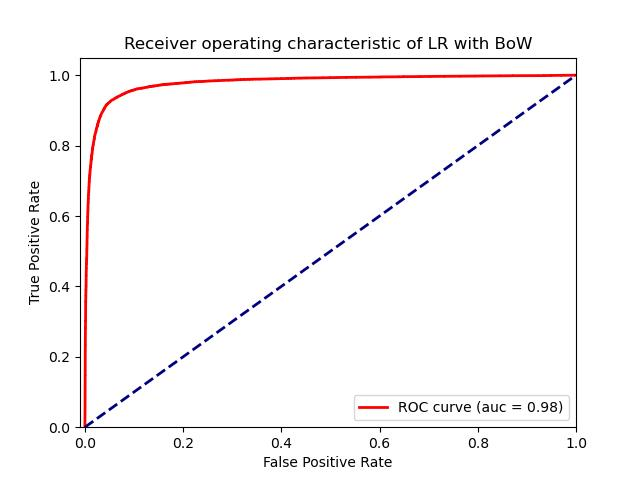
\includegraphics[width=0.4\linewidth]{../img/roc_LR_c.jpg}
            \label{roc_LR_c}}
      \hfil
      \subfloat[LR with Bert Embedding]{
            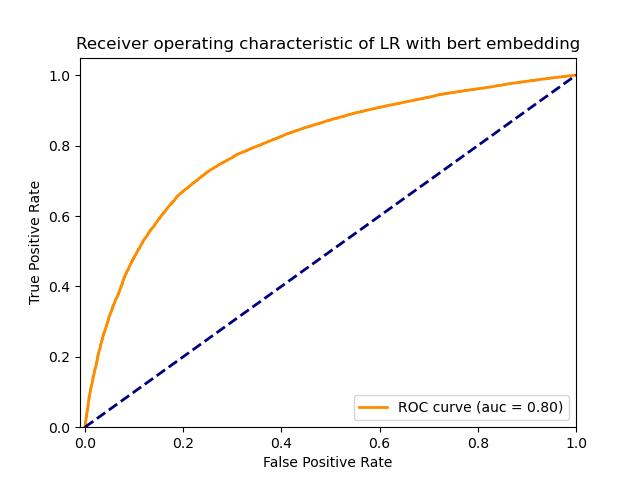
\includegraphics[width=0.4\linewidth]{../img/roc_LR_b.jpg}
            \label{roc_LR_b}}
      \hfil
      \subfloat[LSTM]{
            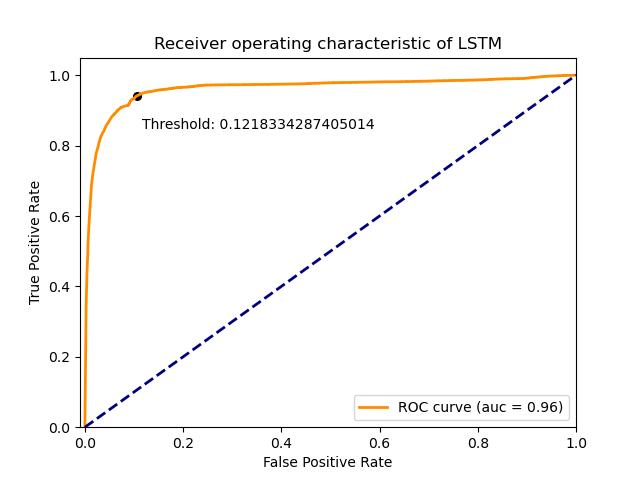
\includegraphics[width=0.4\linewidth]{../img/roc_LSTM.jpg}
            \label{roc_LSTM}}
      \hfil
      \subfloat[BERT]{
            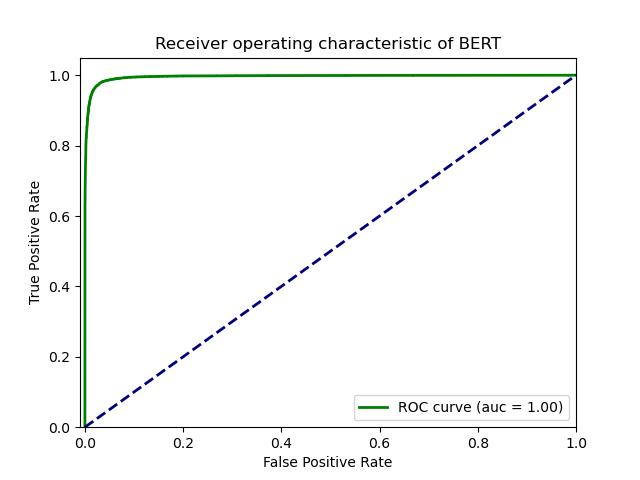
\includegraphics[width=0.4\linewidth]{../img/roc_BERT.jpg}
            \label{roc_BERT}}
      \caption{ROC Curves of Different Models}
      \label{fig:rocs}
\end{figure}

The initial page, as shown in the Figure \ref{fig:pageinitial}, includes an input box, a prediction button, and a button to clear the input. The input box has a default text that prompts the user to enter to the text to be predicted for suicide ideation. After entering the text in the input box, clicking the 'Predict emotions' button, the result of prediction will be shown in the web page.

\begin{figure}[h]
      \centering
      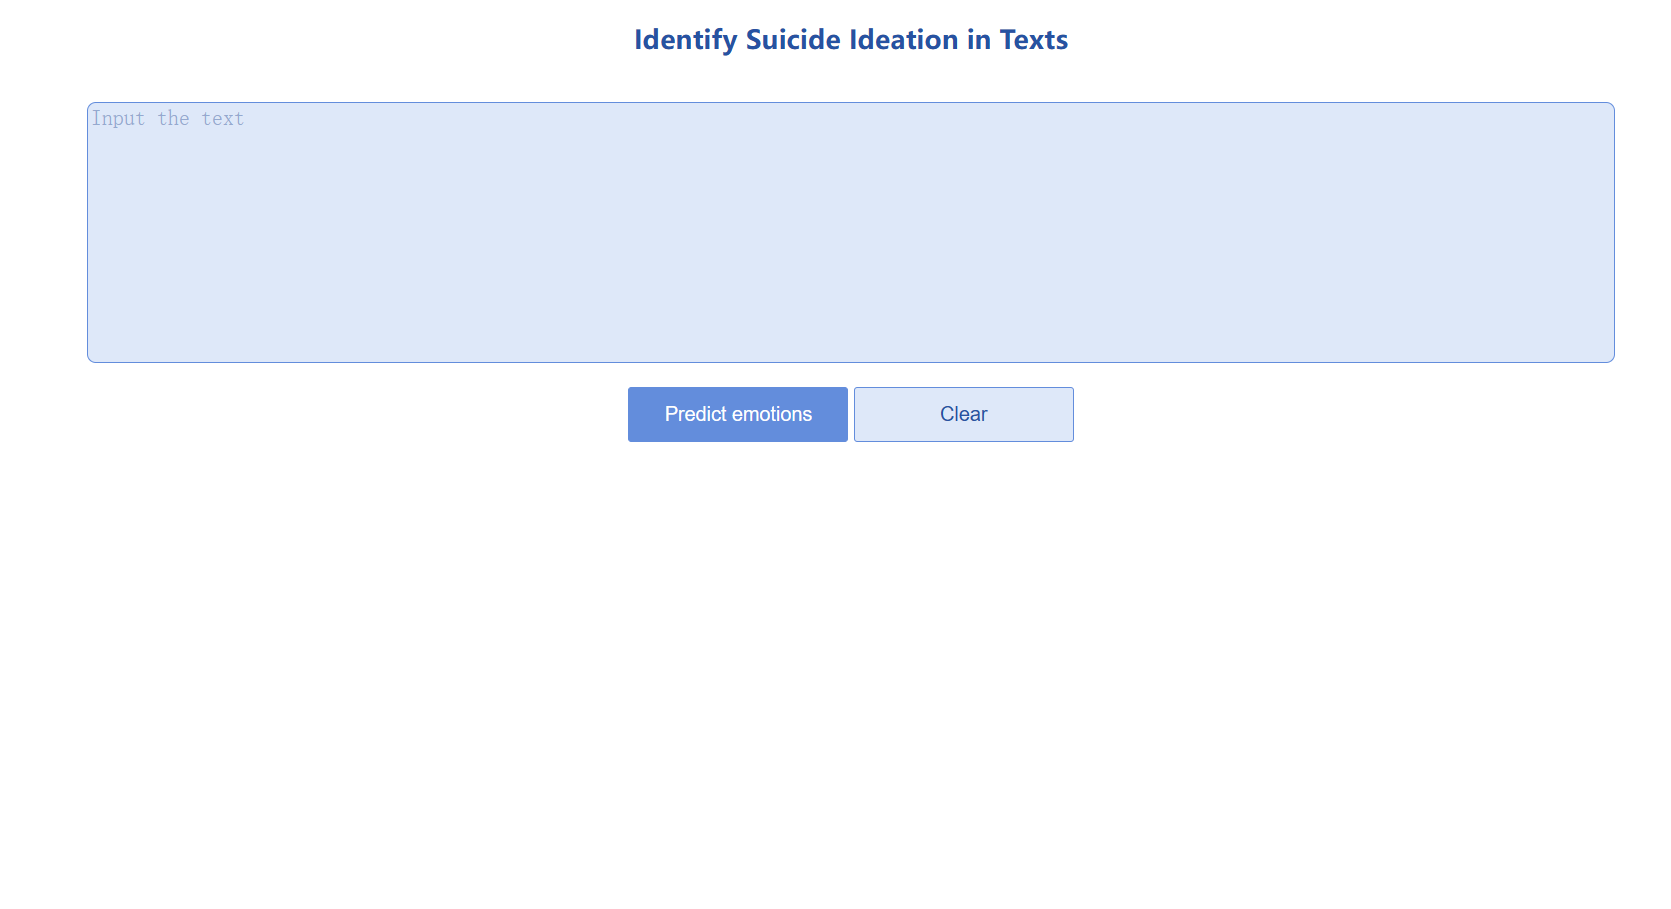
\includegraphics[width=0.57\linewidth]{../img/page_initial.png}
      \caption{Initial Web Page}
      \label{fig:pageinitial}
\end{figure}

The Figure \ref{fig:pagenon} depicts the outcome when the model predicts that the text is not suicidal. The page displays the results of the prediction and indicates the likelihood of the prediction containing suicide ideation.

\begin{figure}[h]
      \centering
      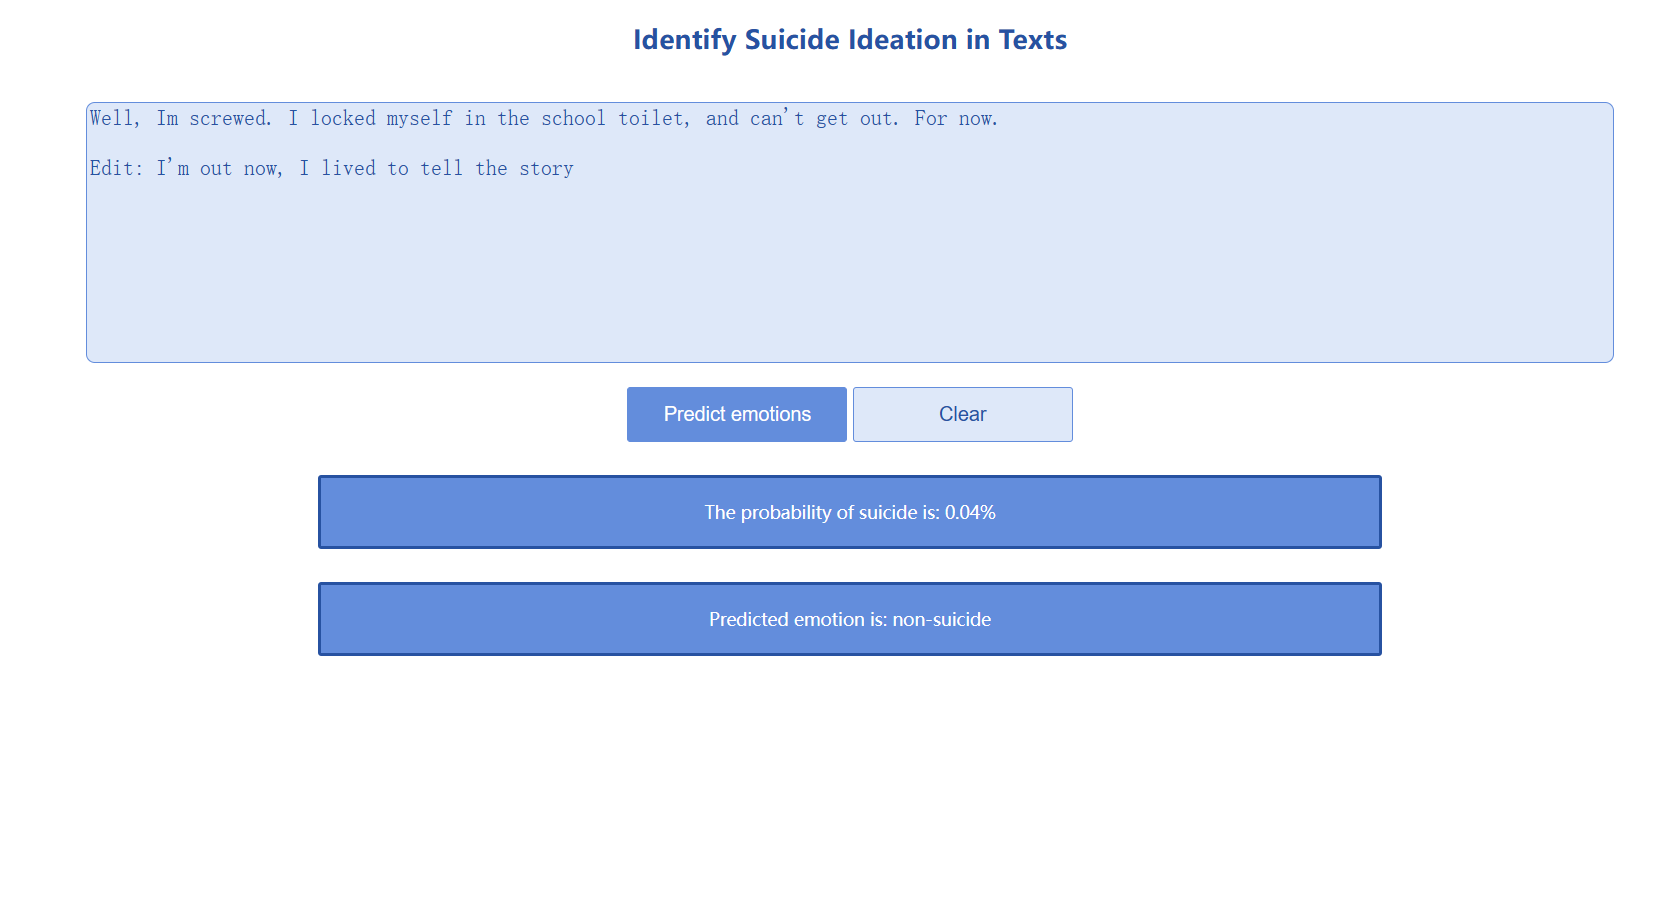
\includegraphics[width=0.57\linewidth]{../img/page_nonsuicide.png}
      \caption{Web Page Showing non-suicide Result}
      \label{fig:pagenon}
\end{figure}

When the model predicts that the text contains suicide ideation, the interface looks as shown in the Figure \ref{fig:pagesui}. The page not only displays the prediction results and the likelihood of containing suicide ideation, it also displays a warning statement, and the alert boxes all turn red to serve as a warning.

\begin{figure}[h]
      \centering
      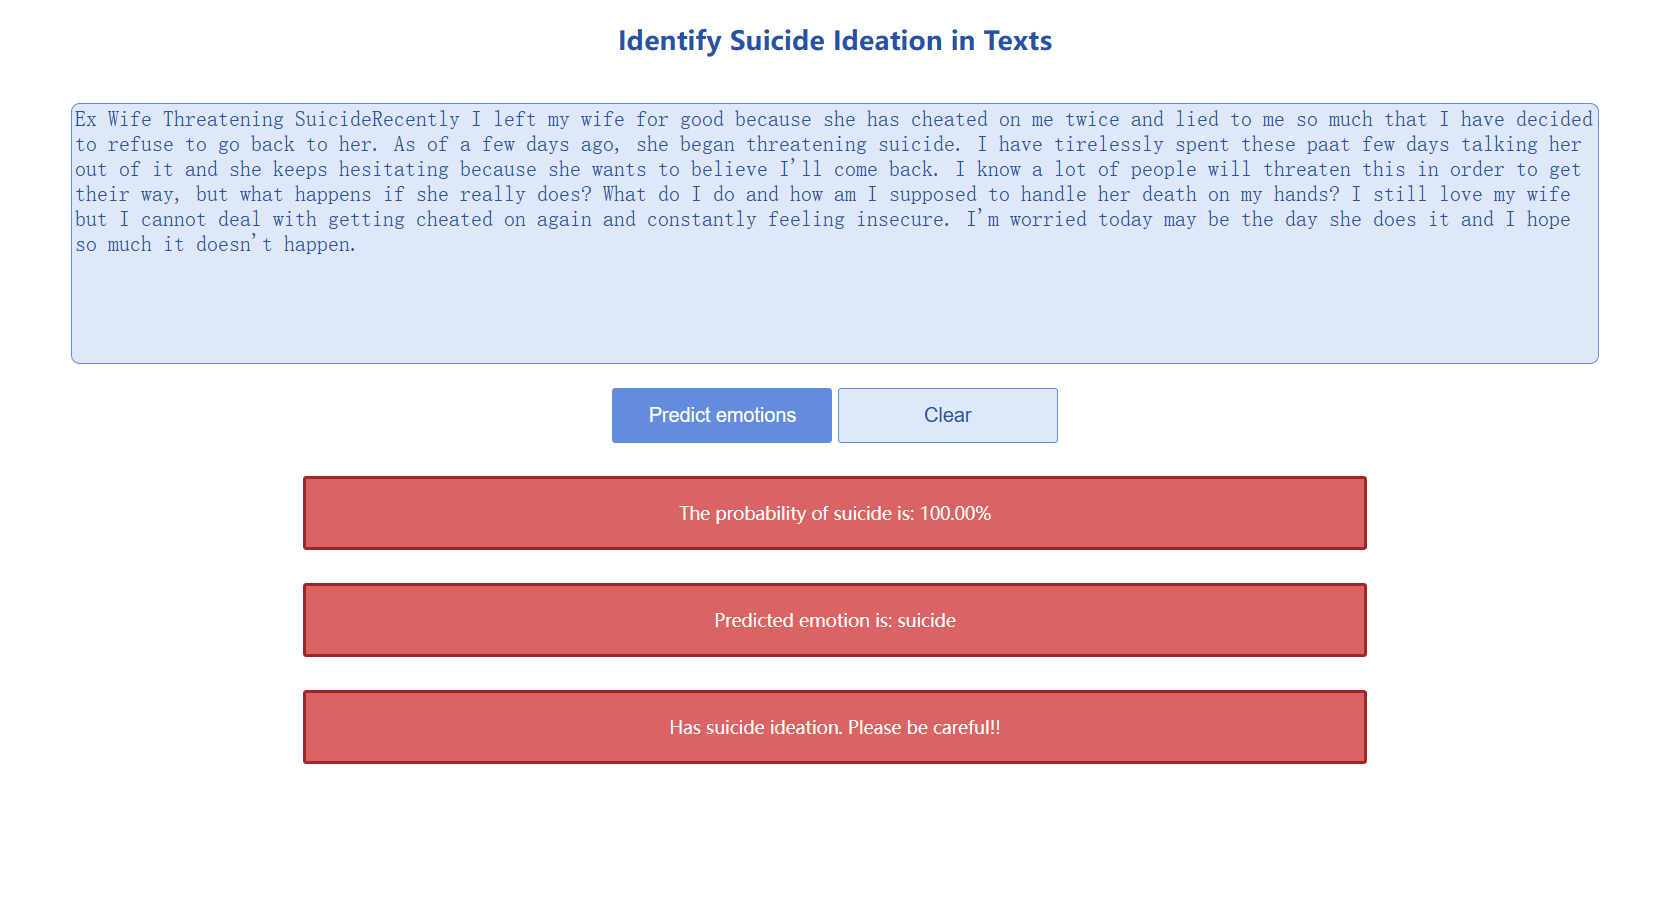
\includegraphics[width=0.57\linewidth]{../img/page_suicide.png}
      \caption{Web Page Showing suicide Result}
      \label{fig:pagesui}
\end{figure}

% -----------------------------------------------------------------------------

\chapter{Conclusion}
\label{chap:conclusion}
\noindent
This chapter will recap the content of the previous chapters, and also present an outline of the main contributions of this project.

\section{Summary}
\noindent
In this era full of network atmosphere, an increasing number of Internet users express their opinions and comments on online social media. At the same time, there is a growing tendency for people to inadvertently express their negative emotions through text. Therefore, it is crucial to perform effective sentiment analysis on textual data that contain personal sentiment information.

This thesis addresses a pressing issue by proposing a model designed to accurately predict whether a text contains suicide ideation. A comparative evaluation of multiple models has been conducted to this end.

Firstly, logistic regression served as the baseline model, followed by the application of both BoW and word embedding techniques. The BoW model achieved an accuracy of 93.26\%, whereas the word embedding approach had a comparatively lower accuracy of only 75.77\%. This illustrates the limitations of simpler models in handling complex contextual information, and therefore more sophisticated models were considered to enhance the accuracy of the predictions.

Subsequently, a variant of RNN: the Bi-LSTM model is considered. This model is able to obtain word associations from both preceding and subsequent text, enhancing feature extraction and elevating the prediction accuracy to 94.79\%. Finally, a pre-trained large language model, BERT, is utilized to replace the traditional neural networks with a more complex architecture for prediction. This approach achieved a remarkable accuracy of 97.28\%, proving that BERT can indeed have superior performance in sentiment classification. Table \ref{tab:performancemetrics} demonstrates a comparison of the performance metrics of the four models used in this project.

\begin{table}[!h]
      \centering
      \begin{tabular}{c|cccc}
            \hline
            Model & Acc(\%) & Pre(\%) & Rec(\%) & F1(\%) \\
            \hline
            LR with BoW             & 93.51 & 95.56 & 91.28 & 93.37 \\
            LR with bert embedding  & 73.66 & 75.63 & 69.88 & 72.64 \\
            Bi-LSTM                 & 94.79 & 93.66 & 96.09 & 94.86 \\
            BERT                    & \textbf{97.28} & \textbf{97.57} & \textbf{97.00} & \textbf{97.28} \\
            \hline
      \end{tabular}
      \caption{Performance Metrics of four Models}
      \label{tab:performancemetrics}
\end{table}

To make this project more relevant, the model was deployed to a web application. Suicide ideation can be predicted from the input text on a web page. In cases where suicidal tendencies are detected, timely warnings will be issued to intervene in suicide as early as possible, offering assistance to those in need.

\section{Further Work}
\noindent
To fulfill the objectives of the project, extensive efforts were dedicated to training, testing, and tuning the models. However, several aspects were unavoidably omitted due to constraints in time and hardware performance. Despite these limitations, a number of additional work are proposed here that could potentially enhance the quality and scope of this project if given more time or resources.

\textbf{Further experiments on existing models}: Due to hardware limitations, the selected models are all validated with only a few simpler versions. For example, currently there are numerous extended models based on BERT, which have further optimise the training process or the network structure, have been developed, such as RoBERTa, BART and so on. These models introduce various enhancements over the foundational BERT model and may be able to perform better than BERT. It might be possible to explore how different pre-training methods would affect the performance of the suicide ideation Identification task, thus helping future developers in making more informed model selection decisions.

\textbf{Combining different models together}: In addition, all the models used in this project used only a single algorithm, but each network has its limitations. There is a growing trend of combining different network models to surpass the performance of a single one. For instance, integrating BERT with CNN and LSTM could provide a unique perspective on how model performance can be enhanced.

\textbf{Expanding the choice of hyperparameters}: Time constraints also influenced the hyperparameter tuning process, only a subset of hyperparameters were tuned to optimize the performance. The hyperparameter selection was limited to a narrow range, which may not fully capture the broader hyperparameter space that could yield improved results.

\textbf{Applying Adversarial Learning}: During the explanation of the model, it was found that some samples that clearly did not contain suicidal ideation were incorrectly judged to be in the suicidal category. And changing just one punctuation could make a huge difference in the prediction result, which is very consistent with the characteristics of the adversarial samples. Adversarial learning\cite{2013Intriguing} can be added to the training process to effectively avoid that "small perturbations" can have a huge impact on the model output. It improves the robustness and safety of the model.

\textbf{Deploying models with more practical implications}: Lastly, the model deployment is relatively straightforward. However, there is significant potential for more sophisticated deployment strategies. The model could be deployed on a cloud service and integrated with other applications to automatically detect and analyze published text. In case where early warnings of suicide ideation are detected, system could provide immediate feedback to the backend system, enabling timely suicide intervention.

% =============================================================================

% Finally, after the main matter, the back matter is specified.  This is
% typically populated with just the bibliography.  LaTeX deals with these
% in one of two ways, namely
%
% - inline, which roughly means the author specifies entries using the 
%   \bibitem macro and typesets them manually, or
% - using BiBTeX, which means entries are contained in a separate file
%   (which is essentially a database) then imported; this is the 
%   approach used below, with the databased being dissertation.bib.
%
% Either way, the each entry has a key (or identifier) which can be used
% in the main matter to cite it, e.g., \cite{X}, \cite[Chapter 2}{Y}.

\backmatter

\bibliography{sample_bibtex.bib}

% -----------------------------------------------------------------------------

% The dissertation concludes with a set of (optional) appendices; these are 
% the same as chapters in a sense, but once signalled as being appendices via
% the associated macro, LaTeX manages them appropriately.

% \appendix

% \chapter{Appendix}
% \label{appx:example}

% Content which is not central to, but may enhance the dissertation can be 
% included in one or more appendices; examples include, but are not limited
% to

% \begin{itemize}
% \item lengthy mathematical proofs, numerical or graphical results which 
%       are summarised in the main body,
% \item sample or example calculations, 
%       and
% \item results of user studies or questionnaires.
% \end{itemize}

% \noindent
% Note that in line with most research conferences, the examiners are not
% obliged to read such appendices.

% =============================================================================

\end{document}
